% Copyright 2007 by Till Tantau
% Copyright 2014 by Rich Wareham, Filippo Spiga
% Copyright 2016 by Petar Veličković
%
% This file may be distributed and/or modified:
% 1. under the LaTeX Project Public License and/or
% 2. under the GNU Public License.
%
% See the file LICENSE for more details.

\documentclass{beamer}

\usetheme{cambridge} 

\setbeamertemplate{navigation symbols}{}  % suppress navigation symbols

%%% Standard packages:
\usepackage[english]{babel}
\usepackage[latin1]{inputenc}
\usepackage{graphicx}
\usepackage{multicol}
\usepackage{subfigure}
\usepackage{listings}
\usepackage{epsfig,setspace,tabularx,xspace}
\usepackage[UKenglish]{isodate}
\usepackage{pgfplots}
\usepackage{bm}
\usepackage{relsize}
\usepackage{rotating}

% Setup TikZ

\usepackage{tikz}
\usetikzlibrary{matrix, arrows, decorations.pathmorphing, shapes}
\usetikzlibrary{positioning, calc, decorations, decorations.pathreplacing}
\tikzstyle{block}=[draw opacity=0.7,line width=1.4cm]

\cleanlookdateon

\newcommand{\argmax}{\operatornamewithlimits{argmax}}
\newcommand{\Proba}{\mathbb{P}}
\newcommand{\tikzmark}[1]{\tikz[overlay,remember picture] \node (#1) {};}

% Author, Title, etc.

\title[Cross-modal convnets] 

}

\author[Veli\v{c}kovi\'{c} et al.]
{
  Petar Veli\v{c}kovi\'{c}
}

\institute[CL]
{Artificial Intelligence Group\\
Computer Laboratory, University of Cambridge, UK}

\date[ARMRS2016]
{Research Students Lecture Series \hfill 21 February 2017}

% The main document

\begin{document}

\begin{frame}
  \titlepage
\end{frame}

\section{Introduction}

\begin{frame}
	\frametitle{Introduction}
	\begin{itemize}
		\item In this lecture, I will introduce \emph{recurrent neural networks} from essential first concepts.
		\vfill
		\item This will cover the application of simple RNNs to solve sequential problems\dots
		\vfill
		\item \dots followed by a deep sweep through \emph{long short-term memories} (LSTMs)\dots
		\vfill
		\item \dots concluding with a variety of modern tips `n' tricks for deploying LSTMs, along with a neat demo (\emph{time permitting}).
		\vfill
		\item Let's get started!
	\end{itemize}
\end{frame}

\begin{frame}
	\frametitle{The three ``flavours'' of machine learning}
	\begin{itemize}
		\item Unsupervised learning
		\vfill
		\item \underline{Supervised} learning\\ \emph{(the only kind of learning neural networks can directly do!)}
		\vfill
		\item Reinforcement learning
	\end{itemize}
\end{frame}

\begin{frame}
	\frametitle{Supervised learning}
	\begin{itemize}
		\item The environment gives you \emph{labelled data} ($\sim$ known \emph{input/output pairs})---and asks you to learn the underlying function.
		\vfill
		\begin{center}
		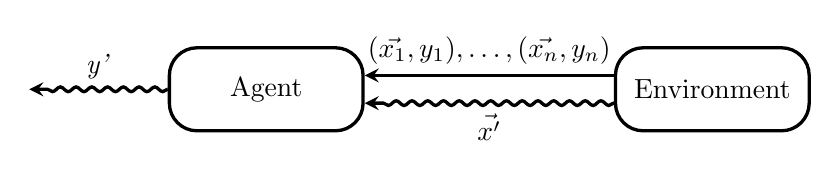
\begin{tikzpicture}
			\node[rectangle, very thick, rounded corners=10, minimum height=3em, minimum width=7em, draw] (lrn) {Agent};
			
			\node[rectangle, very thick, rounded corners=10, minimum height=3em, minimum width=7em, right=9em of lrn, draw] (env) {Environment};
			
			\draw[-stealth, very thick] ([yshift=+0.5em]env.west) -- node[above] {$(\vec{x_1}, y_1), \dots, (\vec{x_n}, y_n)$} ([yshift=+0.5em]lrn.east);
			
			
			\draw[-stealth, decoration={snake, pre length=0.01mm, segment length=2mm, amplitude=0.3mm, post length=1.5mm}, decorate,very thick] ([yshift=-0.5em]env.west) -- node[below] {$\vec{x'}$} ([yshift=-0.5em]lrn.east);
			
			\draw[-stealth, decoration={snake, pre length=0.01mm, segment length=2mm, amplitude=0.3mm, post length=1.5mm}, decorate,very thick] (lrn.west) -- node[above] {\emph{y'}} ([xshift=-5em]lrn.west);
		\end{tikzpicture}
		\end{center}
		\vfill
		\item Example: determining whether a person will be likely to return their loan, given their credit history (and a set of previous data on issued loans to other customers).
	\end{itemize}
\end{frame}

\begin{frame}
	\frametitle{Classification}
	\begin{itemize}
		\item Specifically, we will focus on \emph{classification}---assuming our outputs to come from a discrete set of \emph{classes}.
	\end{itemize}
	\vfill
	\begin{center}
	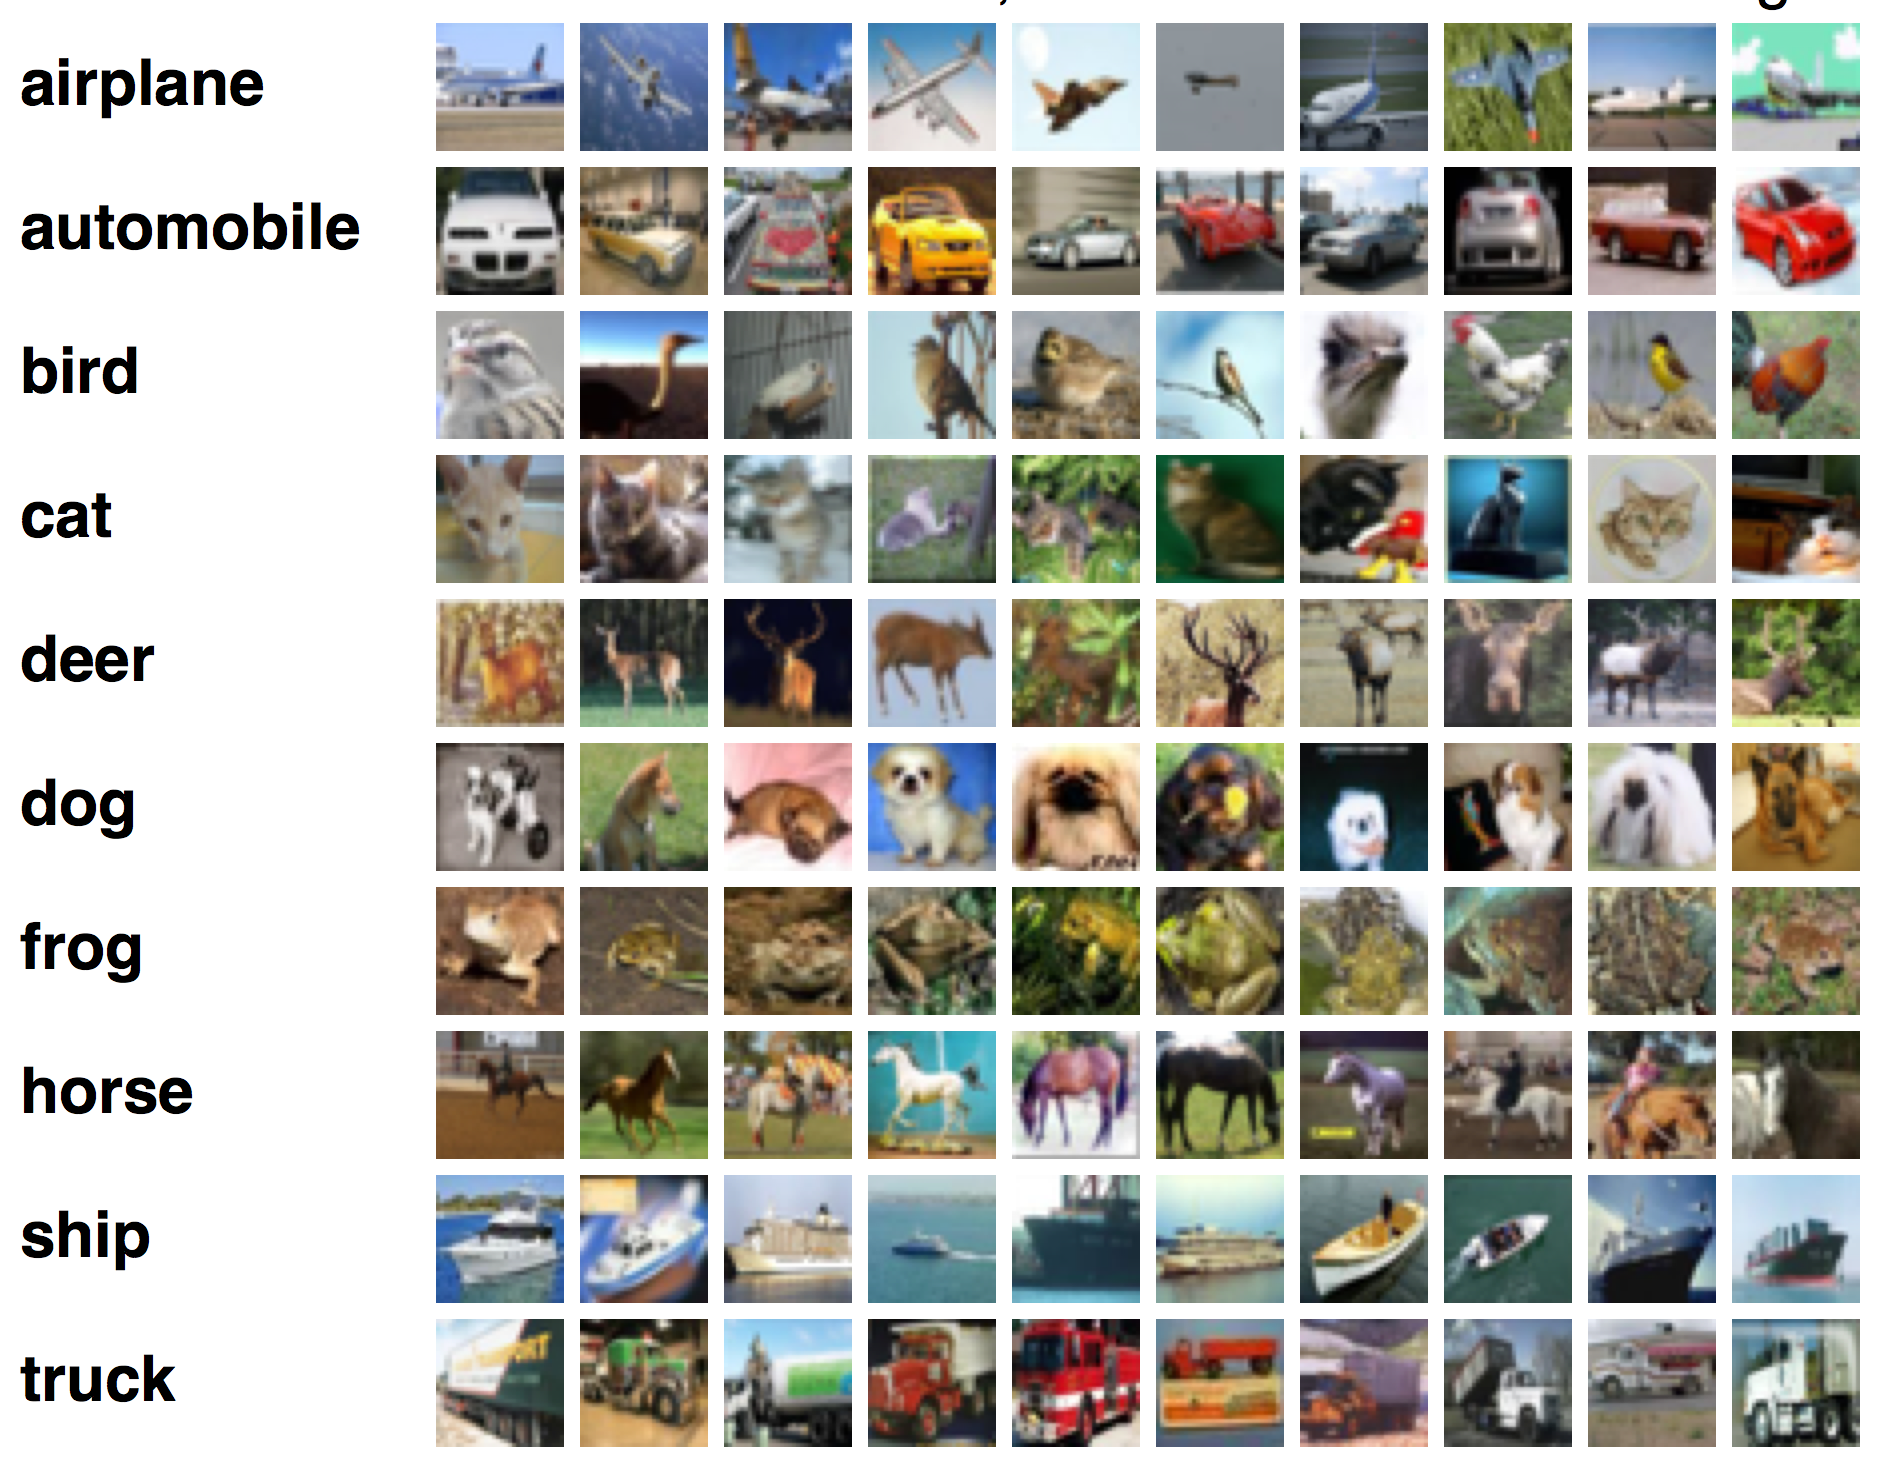
\includegraphics[width=0.6\linewidth]{CIFAR-10.png}
	\end{center}
\end{frame}

\section{Simple NN classifiers}

\begin{frame}
	\frametitle{Neural networks}
	\begin{itemize}
		\item To make life simpler (esp. notationally!), let's start with an introduction to simple neural networks.
		\vfill
		\item \textbf{Neural networks} are structures of interconnected processing units (\emph{neurons}).	
		\vfill
		\item Each neuron computes a linear combination of its \emph{inputs}, afterwards potentially applying an \emph{activation function}, to produce its \emph{output}.
		\vfill
		\item Occasionally, I will illustrate how to specify neural networks of interest using \emph{Keras} ({\tt keras.io}). (\textbf{highly recommended!})
	\end{itemize}
\end{frame}

\begin{frame}
	\frametitle{A single neuron}
	Within this context sometimes also called a \emph{perceptron} (\dots)
	\vfill
	\tikzstyle{inputNode}=[draw,circle,minimum size=10pt,inner sep=0pt]
\tikzstyle{stateTransition}=[-stealth, thick]
\begin{center}
\scalebox{0.95}{%
\begin{tikzpicture}
	\node[draw,circle,minimum size=25pt,inner sep=0pt] (x) at (0,0) {$\Sigma$ $\sigma$};

	\node[inputNode] (x0) at (-2, 1.5) {$\tiny +1$};
	\node[inputNode] (x1) at (-2, 0.75) {$\tiny x_1$};
	\node[inputNode] (x2) at (-2, 0) {$\tiny x_2$};
	\node[inputNode] (x3) at (-2, -0.75) {$\tiny x_3$};
	\node[inputNode] (xn) at (-2, -1.75) {$\tiny x_n$};

	\draw[stateTransition] (x0) to[out=0,in=120] node [midway, sloped, above] {$b$} (x);
	\draw[stateTransition] (x1) to[out=0,in=150] node [midway, sloped, above] {$w_1$} (x);
	\draw[stateTransition] (x2) to[out=0,in=180] node [midway, sloped, above] {$w_2$} (x);
	\draw[stateTransition] (x3) to[out=0,in=210] node [midway, sloped, above] {$w_3$} (x);
	\draw[stateTransition] (xn) to[out=0,in=240] node [midway, sloped, above] {$w_n$} (x);
	\draw[stateTransition] (x) -- (5,0) node [midway,above] {$h(\vec{x}; \vec{w}) = \sigma\left(b + \sum\limits_{i=1}^{n}{w_ix_i}\right)$};
	\draw[dashed] (0,-0.43) -- (0,0.43);
	\node (dots) at (-2, -1.15) {$\vdots$};
\end{tikzpicture}}
\end{center}
\vfill
Popular choices for the activation function $\sigma$:
\begin{itemize}
	\item \emph{Identity}: $\sigma(x) = x$;
	\item \emph{Rectified linear unit (ReLU)}: $\sigma(x) = \max(0, x)$;
	\item \emph{Sigmoid functions}: $\sigma(x) = \frac{1}{1 + \exp(-x)}$ (\emph{logistic}); $\sigma(x) = \tanh{x}$.
\end{itemize}
\end{frame}

\begin{frame}
	\frametitle{Activation functions}
	\centering
	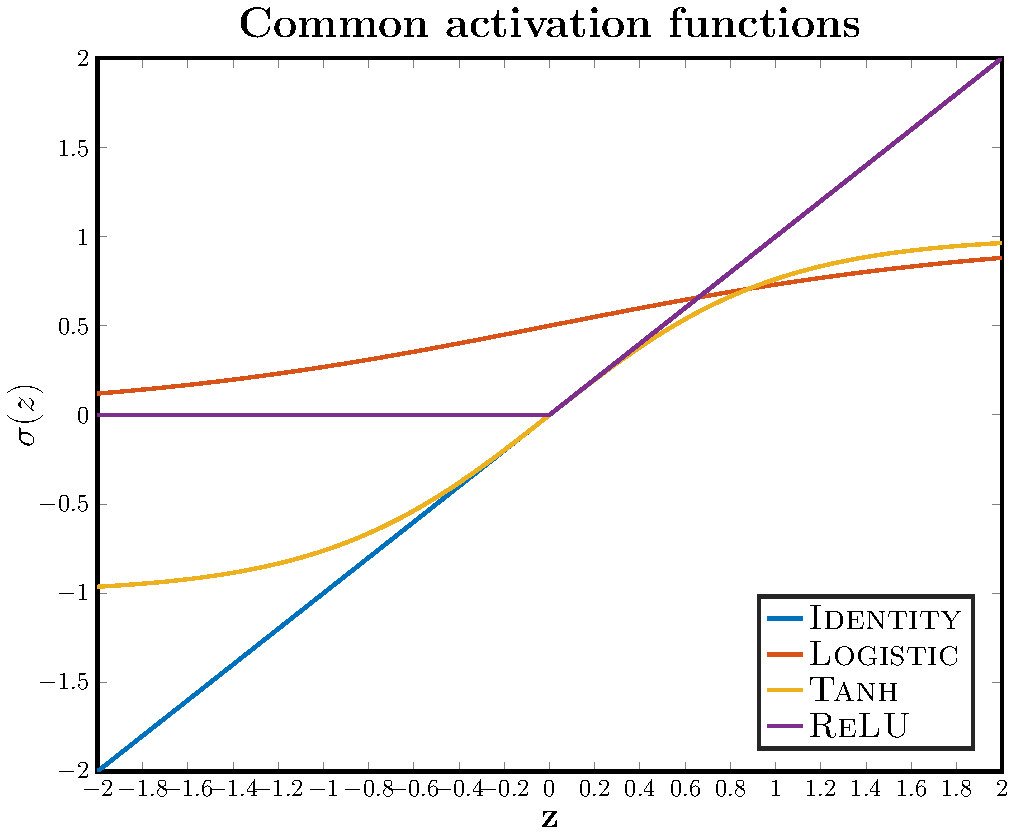
\includegraphics[width=0.7\linewidth]{plotker.pdf}
\end{frame}

\begin{frame}
	\frametitle{Neural networks and deep learning}
	\begin{itemize}
		\item It is easy to extend a single neuron to a \emph{neural network}---simply connect outputs of neurons to inputs of other neurons. 
		\vfill
		\item We may do this in two ways:
		\begin{itemize}
			\item \textbf{Feedforward}: the computation graph does not have cycles;
			\item \textbf{Recurrent}: the computation graph has cycles.
		\end{itemize}
		\vfill
		\item Typically we organise neural networks in a sequence of \emph{layers}, such that a single layer only processes output from the previous layer. Everything with $>1$ hidden layer is \emph{``deep''}!
	\end{itemize}
\end{frame}

\begin{frame}
	\frametitle{A few details on training}
	\begin{itemize}
		\item Neural networks are trained from known (input, output) samples. The training algorithm adapts the neurons' weights to maximise \emph{predictive power} on the training examples. 
		\vfill
		\item This is done, for a single training example $(\vec{x}, y)$, by:
		\begin{itemize} 
			\item Computing the output of the network $y' = h(\vec{x}; \vec{w})$;
			\item Determining the \emph{loss} of this output $\mathcal{L}(y, y')$;
			\item Computing partial derivatives of the loss with respect to each weight, $\frac{\partial\mathcal{L}}{\partial \vec{w}}$, and using these to update weights.
			\item Key words: \emph{backpropagation}, \emph{stochastic gradient descent}.
		\end{itemize}
	\end{itemize}
\end{frame}

\begin{frame}
	\frametitle{A simple classifier}
	Let's ignore the activation functions and ``deep learning'' for now\dots here is a simple, shallow, 4-class classifier.
	\vfill
		\tikzstyle{inputNode}=[draw,circle,minimum size=10pt,inner sep=0pt]
\tikzstyle{stateTransition}=[-stealth, thick]
	\begin{center}
\scalebox{0.95}{%
\begin{tikzpicture}
	\node[draw,circle,minimum size=15pt,inner sep=0pt] (o1) at (0,0.9) {$\Sigma$};
	\node[draw,circle,minimum size=15pt,inner sep=0pt] (o2) at (0,0.3) {$\Sigma$};
	\node[draw,circle,minimum size=15pt,inner sep=0pt] (o3) at (0,-0.3) {$\Sigma$};
	\node[draw,circle,minimum size=15pt,inner sep=0pt] (o4) at (0,-0.9) {$\Sigma$};

	\node[inputNode] (x0) at (-2, 1.5) {$\tiny +1$};
	\node[inputNode] (x1) at (-2, 0.75) {$\tiny x_1$};
	\node[inputNode] (x2) at (-2, 0) {$\tiny x_2$};
	\node[inputNode] (x3) at (-2, -0.75) {$\tiny x_3$};
	\node[inputNode] (xn) at (-2, -1.75) {$\tiny x_n$};

	\draw[stateTransition] (x0) to[] (o1);
	\draw[stateTransition] (x1) to[] (o1);
	\draw[stateTransition] (x2) to[] (o1);
	\draw[stateTransition] (x3) to[] (o1);
	\draw[stateTransition] (xn) to[] (o1);
	\draw[stateTransition] (x0) to[] (o2);
	\draw[stateTransition] (x1) to[] (o2);
	\draw[stateTransition] (x2) to[] (o2);
	\draw[stateTransition] (x3) to[] (o2);
	\draw[stateTransition] (xn) to[] (o2);
	\draw[stateTransition] (x0) to[] (o3);
	\draw[stateTransition] (x1) to[] (o3);
	\draw[stateTransition] (x2) to[] (o3);
	\draw[stateTransition] (x3) to[] (o3);
	\draw[stateTransition] (xn) to[] (o3);
	\draw[stateTransition] (x0) to[] (o4);
	\draw[stateTransition] (x1) to[] (o4);
	\draw[stateTransition] (x2) to[] (o4);
	\draw[stateTransition] (x3) to[] (o4);
	\draw[stateTransition] (xn) to[] (o4);
	\draw[stateTransition] (o1) -- (1.5,0.9);
	\draw[stateTransition] (o2) -- (1.5,0.3);
	\draw[stateTransition] (o3) -- (1.5,-0.3);
	\draw[stateTransition] (o4) -- (1.5,-0.9);
	\node (dots) at (-2, -1.15) {$\vdots$};
\end{tikzpicture}}
\end{center}
\vfill
Choose the class which has the maximal \emph{output}:
\begin{center}$C = \argmax_j \left\{b_j + \sum_{i=1}^{n} w_{ij}x_i\right\}$\end{center}

\end{frame}

\begin{frame}
	\frametitle{Block notation}
	Note that this layer is essentially doing a matrix multiplication\dots
	\vfill
		\tikzstyle{inputNode}=[draw,circle,minimum size=10pt,inner sep=0pt]
\tikzstyle{stateTransition}=[-stealth, thick]
	\begin{center}
\scalebox{0.95}{%
\begin{tikzpicture}
	
	\node[rectangle, draw, minimum width=0.5cm,minimum height=2.5cm] (X) at (-2, 0) {$\vec{x}$};
	
	\node[rectangle, draw, right=of X, text depth=0em, minimum width=1.5cm,minimum height=2.5cm] (W) {${\bf W}\times$};

	\node[rectangle, draw, right=of W, text depth=0em, minimum width=0.5cm,minimum height=1.5cm] (B) {$+ \vec{b}$};
	
	\node[rectangle, right=of B] (out) {};
	
	\foreach \x in {1,...,3}
    		\draw[stateTransition] ([yshift=\x em]X.east) -- ([yshift=\x em]W.west);
    \foreach \x in {1,...,3}
    		\draw[stateTransition] ([yshift=-\x em]X.east) -- ([yshift=-\x em]W.west);
	\draw[-stealth, thick] (X) -- (W);
	
	\foreach \x in {-1.5, -0.5, 0.5, 1.5}
    		\draw[stateTransition] ([yshift=\x em]W.east) -- ([yshift=\x em]B.west);
	\foreach \x in {-1.5, -0.5, 0.5, 1.5}
    		\draw[stateTransition] ([yshift=\x em]B.east) -- ([yshift=\x em]out.west);
	
\end{tikzpicture}}
\end{center}
\vfill
\begin{center}$C = \argmax_j \left({\bf W}\vec{x} + \vec{b}\right)_j$\end{center}
{\bf N.B.} $\bf W$ of size $4 \times n$, $\vec{b}$ of size $4$!
\end{frame}


\begin{frame}
	\frametitle{Softmax}
	\begin{itemize}
		\item \textbf{Problem}: what should the targets be?
		\vfill
		\item Outputs are \emph{unbounded}! For an example of the second class, the targets should be $\vec{y} = \begin{bmatrix}-\infty\ & +\infty\ & -\infty\ & -\infty\end{bmatrix}$\dots
		\vfill
		\item \textbf{Solution}: transform the outputs monotonically to the $[0, 1]$ range, using the \emph{softmax} function:
		\[softmax(\vec{z})_i = \frac{\exp(z_i)}{\sum_j \exp(z_j)}\]
	\end{itemize}
\end{frame}

\begin{frame}
	\frametitle{Probabilistic classification}
	\begin{itemize}
		\item This conveniently also makes the outputs add up to $1$, so we can interpret $y'_i = softmax(h(\vec{x}))_i = \mathbb{P}(\vec{x}\ in\ class\ i)$.
		\vfill
		\item Now the target for an example of the second class should be $\vec{y} = \begin{bmatrix}0 & 1 & 0 & 0\end{bmatrix}$ ($\sim$ one-hot encoding).
		\vfill
		\item Typically express the loss function as the \emph{cross-entropy}:
		\[\mathcal{L}(\vec{y}, \vec{y}') = \sum_{i=1}^K y_i \log y'_i\]
		where $K$ is the number of classes.
	\end{itemize}
\end{frame}

\begin{frame}
	\frametitle{Back in business}
	Integrating into our simple classifier:
	\vfill
		\tikzstyle{inputNode}=[draw,circle,minimum size=10pt,inner sep=0pt]
\tikzstyle{stateTransition}=[-stealth, thick]
	\begin{center}
\scalebox{0.95}{%
\begin{tikzpicture}
	
	\node[rectangle, draw, minimum width=0.5cm,minimum height=2.5cm] (X) at (-2, 0) {$\vec{x}$};
	
	\node[rectangle, draw, right=of X, text depth=0em, minimum width=1.5cm,minimum height=2.5cm] (W) {${\bf W}\times$};

	\node[rectangle, draw, right=of W, text depth=0em, minimum width=0.5cm,minimum height=1.5cm] (B) {$+ \vec{b}$};
	
	\node[right=of B, inner sep=0em] (out) {
	\begin{tikzpicture}
		\node[rectangle, draw, rotate=90, minimum height=0.5cm, minimum width=1.5cm] (out) {$softmax$};
	\end{tikzpicture}
	};
	
	\node[right=of out] (outt) {};
	
	\foreach \x in {1,...,3}
    		\draw[stateTransition] ([yshift=\x em]X.east) -- ([yshift=\x em]W.west);
    \foreach \x in {1,...,3}
    		\draw[stateTransition] ([yshift=-\x em]X.east) -- ([yshift=-\x em]W.west);
	\draw[-stealth, thick] (X) -- (W);
	
	\foreach \x in {-1.5, -0.5, 0.5, 1.5}
    		\draw[stateTransition] ([yshift=\x em]W.east) -- ([yshift=\x em]B.west);
	\foreach \x in {-1.5, -0.5, 0.5, 1.5}
    		\draw[stateTransition] ([yshift=\x em]B.east) -- ([yshift=\x em]out.west);
	\foreach \x in {-1.5, -0.5, 0.5, 1.5}
    		\draw[stateTransition] ([yshift=\x em]out.east) -- ([yshift=\x em]outt.west);
	
\end{tikzpicture}}
\end{center}
\vfill
\begin{center}$C = \argmax_j \left\{softmax\left({\bf W}\vec{x} + \vec{b}\right)_j\right\}$\end{center}
\end{frame}

\begin{frame}
	\frametitle{Going deeper with LEGO\textsuperscript{TM}}
	Making things \emph{deep} is now easy\dots
	\vfill
		\tikzstyle{inputNode}=[draw,circle,minimum size=10pt,inner sep=0pt]
\tikzstyle{stateTransition}=[-stealth, thick]
	\begin{center}
\scalebox{0.95}{%
\begin{tikzpicture}
	
	\node[rectangle, draw, minimum width=0.5cm,minimum height=2.5cm] (X) at (-2, 0) {$\vec{x}$};
	
	\node[rectangle, draw, right=1.5em of X, text depth=0em, minimum width=1.5cm,minimum height=2.5cm] (W1) {${\bf W_1}\times$};

	\node[rectangle, draw, right=1.5em of W1, text depth=0em, minimum width=0.5cm,minimum height=2.5cm] (B1) {$+ \vec{b}_1$};
	
	\node[rectangle, draw, right=1.5em of B1, text depth=0em, minimum width=1.5cm,minimum height=2.5cm] (RL) {
		\begin{tikzpicture}
			\draw[thick] (0,0) -- (0.5, 0);
			\draw[thick] (0.49,-0.004) -- (0.99, 0.496);
		\end{tikzpicture}
	};
	
	\node[rectangle, draw, right=1.5em of RL, text depth=0em, minimum width=1.5cm,minimum height=2.5cm] (W) {${\bf W_2}\times$};

	\node[rectangle, draw, right=1.5em of W, text depth=0em, minimum width=0.5cm,minimum height=1.5cm] (B) {$+ \vec{b}_2$};
	
	\node[right=1.5em of B, inner sep=0em] (out) {
	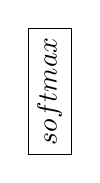
\begin{tikzpicture}
		\node[rectangle, draw, rotate=90, minimum height=0.5cm, minimum width=1.5cm] (out) {$softmax$};
	\end{tikzpicture}
	};
	
	\node[right=1.5em of out] (outt) {};
	
	\foreach \x in {1,...,3}
    		\draw[stateTransition] ([yshift=\x em]X.east) -- ([yshift=\x em]W1.west);
    \foreach \x in {1,...,3}
    		\draw[stateTransition] ([yshift=-\x em]X.east) -- ([yshift=-\x em]W1.west);
	\draw[-stealth, thick] (X) -- (W1);
	
	\foreach \x in {1,...,3}
    		\draw[stateTransition] ([yshift=\x em]W1.east) -- ([yshift=\x em]B1.west);
    \foreach \x in {1,...,3}
    		\draw[stateTransition] ([yshift=-\x em]W1.east) -- ([yshift=-\x em]B1.west);
	\draw[-stealth, thick] (W1) -- (B1);
	
	\foreach \x in {1,...,3}
    		\draw[stateTransition] ([yshift=\x em]B1.east) -- ([yshift=\x em]RL.west);
    \foreach \x in {1,...,3}
    		\draw[stateTransition] ([yshift=-\x em]B1.east) -- ([yshift=-\x em]RL.west);
	\draw[-stealth, thick] (B1) -- (RL);
	
	\foreach \x in {1,...,3}
    		\draw[stateTransition] ([yshift=\x em]RL.east) -- ([yshift=\x em]W.west);
    \foreach \x in {1,...,3}
    		\draw[stateTransition] ([yshift=-\x em]RL.east) -- ([yshift=-\x em]W.west);
	\draw[-stealth, thick] (RL) -- (W);
	
	\foreach \x in {-1.5, -0.5, 0.5, 1.5}
    		\draw[stateTransition] ([yshift=\x em]W.east) -- ([yshift=\x em]B.west);
	\foreach \x in {-1.5, -0.5, 0.5, 1.5}
    		\draw[stateTransition] ([yshift=\x em]B.east) -- ([yshift=\x em]out.west);
	\foreach \x in {-1.5, -0.5, 0.5, 1.5}
    		\draw[stateTransition] ([yshift=\x em]out.east) -- ([yshift=\x em]outt.west);
	
\end{tikzpicture}}
\end{center}
\vfill
\begin{center}$C = \argmax_j \left\{softmax\left({\bf W_2}ReLU\left({\bf W_1}\vec{x} + \vec{b}_1\right) + \vec{b}_2\right)_j\right\}$\end{center}
{\bf N.B.} the ReLU is \emph{important}! A composition of linear functions is itself a linear function\dots
\end{frame}

\begin{frame}
	\frametitle{Fully connected layers}
	The ``matrix-multiply--bias--activation'' (sometimes also called \emph{fully connected} or \texttt{Dense}) layer is a common building block of neural networks.
	\vfill
		\tikzstyle{inputNode}=[draw,circle,minimum size=10pt,inner sep=0pt]
\tikzstyle{stateTransition}=[-stealth, thick]
	\begin{center}
\scalebox{0.95}{%
\begin{tikzpicture}
	
	\node[rectangle, draw, minimum width=0.5cm,minimum height=2.5cm] (X) at (-2, 0) {$\vec{x}$};
	
	\node[rectangle, draw, right= of X, align=center, text depth=0em, minimum width=1.5cm,minimum height=2.5cm] (W1) {{\tt Dense(7)}\\[2ex]\begin{tikzpicture}
			\draw[thick] (0,0) -- (0.5, 0);
			\draw[thick] (0.49,-0.004) -- (0.99, 0.496);
		\end{tikzpicture}};

	\node[rectangle, draw, right= of W1, align=center, text depth=0em, minimum width=0.5cm,minimum height=2.5cm] (W2) {{\tt Dense(4)}\\[2ex]\emph{softmax}};	
	\node[right= of W2] (out) {};
	
	\foreach \x in {1,...,3}
    		\draw[stateTransition] ([yshift=\x em]X.east) -- ([yshift=\x em]W1.west);
    \foreach \x in {1,...,3}
    		\draw[stateTransition] ([yshift=-\x em]X.east) -- ([yshift=-\x em]W1.west);
	\draw[-stealth, thick] (X) -- (W1);
	
	\foreach \x in {1,...,3}
    		\draw[stateTransition] ([yshift=\x em]W1.east) -- ([yshift=\x em]W2.west);
    \foreach \x in {1,...,3}
    		\draw[stateTransition] ([yshift=-\x em]W1.east) -- ([yshift=-\x em]W2.west);
	\draw[-stealth, thick] (W1) -- (W2);
	
	
	\foreach \x in {-1.5, -0.5, 0.5, 1.5}
    		\draw[stateTransition] ([yshift=\x em]W2.east) -- ([yshift=\x em]out.west);
	
\end{tikzpicture}}
\end{center}
\vfill
Keras code:\\
{\small \tt x = Input(shape=(7,))\\
h = Dense(7, activation='relu')(x)\\
y = Dense(4, activation='softmax')(h)}
\end{frame}

\section{SimpleRNN}

\begin{frame}
	\frametitle{Sequential inputs}
	\begin{itemize}
		\item Now, consider a classification problem where the input is \emph{sequential}---a sequence consisting of arbitrarily many \emph{steps}, wherein at each step we have $n$ \emph{features}.
	\end{itemize}
	\begin{center}
		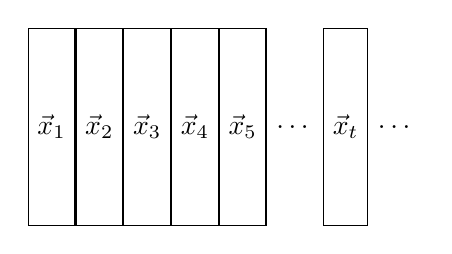
\begin{tikzpicture}
			\node[rectangle, draw, minimum width=0.5cm,minimum height=2.5cm] (X) at (-2, 0) {$\vec{x}_1$};
			\node[rectangle, draw, right=0em of X,minimum width=0.5cm,minimum height=2.5cm] (X) {$\vec{x}_2$};
			\node[rectangle, draw, right=0em of X,minimum width=0.5cm,minimum height=2.5cm] (X)  {$\vec{x}_3$};
			\node[rectangle, draw, right=0em of X,minimum width=0.5cm,minimum height=2.5cm] (X)  {$\vec{x}_4$};
			\node[rectangle, draw, right=0em of X,minimum width=0.5cm,minimum height=2.5cm] (X)  {$\vec{x}_5$};
			\node[right=0em of X] (X) {\dots};
			\node[rectangle, draw, right=0em of X,minimum width=0.5cm,minimum height=2.5cm] (X)  {$\vec{x}_t$};
			\node[right=0em of X] (X) {\dots};
		\end{tikzpicture}
	\end{center}
	\begin{itemize}
		\item The fully connected layers will no longer suffice, as they expect a \emph{fixed-size} input!
	\end{itemize}
\end{frame}

\begin{frame}
	\frametitle{Making it work}
	\textbf{Key} ideas:
	\begin{itemize}
		\item \emph{Summarize} the entire input into $m$ features (describing the most important patterns for classifying it);
		\vfill
		\item Exploit relations between \emph{adjacent steps}---process the input in a \emph{step-by-step} manner, iteratively building up the features, $\vec{h}$:
		\[\vec{h}_t = f(\vec{x}_t, \vec{h}_{t-1})\]
		\vfill
		\item If we declare a pattern to be \emph{interesting}, then it does not matter \textbf{when} it occurs in the sequence $\implies$ employ \emph{weight sharing}!
	\end{itemize}
\end{frame}

\begin{frame}
	\frametitle{An RNN cell}
	\begin{center}
		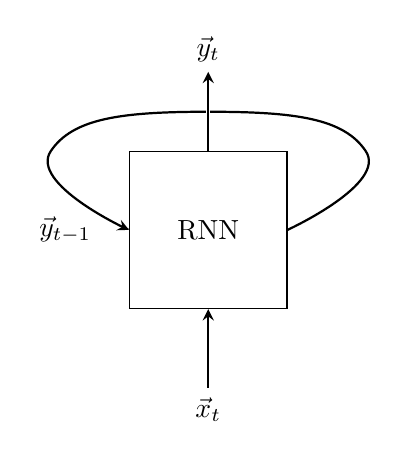
\begin{tikzpicture}
			\node[rectangle, draw, minimum height=2cm, minimum width=2cm] (RNN) at (0, 0) {RNN};
			\node[below=of RNN] (X) {$\vec{x}_t$};
			\node[above=of RNN] (Y) {$\vec{y}_t$};
			\draw[-stealth, thick] (X) -- (RNN);
			\draw [-stealth,thick] plot[smooth,tension=1] coordinates { (RNN.east)  (2,1)  (0,1.5) (-2,1) (RNN.west)} node[left=1em] {$\vec{y}_{t-1}$};
			\draw[-stealth, ultra thick, white] (RNN) -- (Y);
			\draw[-stealth, thick] (RNN) -- (Y);
		\end{tikzpicture}
	\end{center}
\end{frame}

\begin{frame}
	\frametitle{Unrolling the cell\dots}
	\begin{center}
		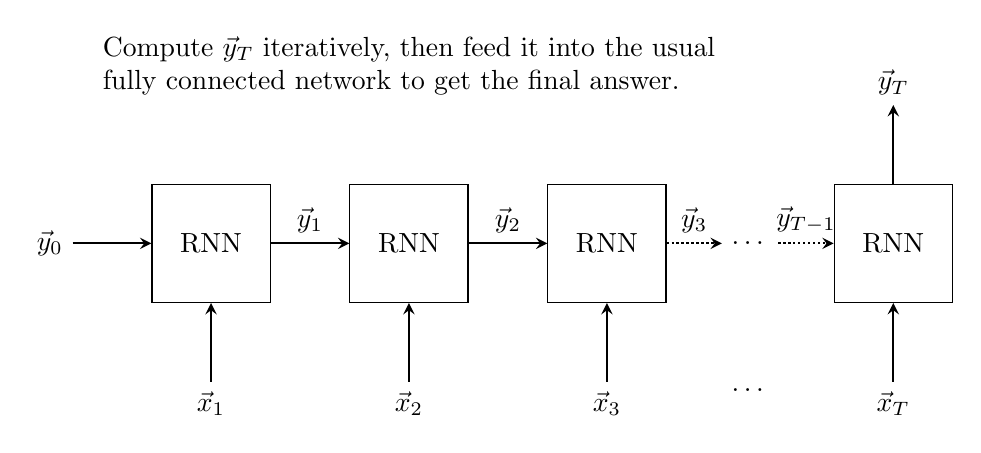
\begin{tikzpicture}
			\node[rectangle, draw, minimum height=1.5cm, minimum width=1.5cm] (RNN) at (0, 0) {RNN};
			\node[rectangle, right=of RNN, draw, minimum height=1.5cm, minimum width=1.5cm] (RNN2) {RNN};
			\node[rectangle, right=of RNN2, draw, minimum height=1.5cm, minimum width=1.5cm] (RNN3) {RNN};
			
			\node[above=of RNN2, align=left] {
	Compute $\vec{y}_T$ iteratively, then feed it into the usual\\ fully connected network to get the final answer.};
			\node[rectangle, right=2em of RNN3] (RNN4) {\dots};
			\node[rectangle, right=2em of RNN4, draw, minimum height=1.5cm, minimum width=1.5cm] (RNN5) {RNN};
			
			\node[below=of RNN] (X1) {$\vec{x}_1$};
			\node[below=of RNN2] (X2) {$\vec{x}_2$};
			\node[below=of RNN3] (X3) {$\vec{x}_3$};
			\node[below=of RNN5] (X4) {$\vec{x}_T$};
			\node[above=of RNN5] (Y) {$\vec{y}_T$};
			\node[left=of RNN] (Y0) {$\vec{y}_0$};
			
			\draw[-stealth, thick] (X1) -- (RNN);
			\draw[-stealth, thick] (X2) -- (RNN2);
			\draw[-stealth, thick] (X3) -- (RNN3);
			\draw[-stealth, thick] (X4) -- (RNN5);
			\draw[-stealth, thick] (Y0) -- (RNN);
			\draw[-stealth, thick] (RNN5) -- (Y);
			\draw[-stealth, thick] (RNN) -- node[above] {$\vec{y}_1$} (RNN2);
			\draw[-stealth, thick] (RNN2) -- node[above] {$\vec{y}_2$} (RNN3);
			\draw[-stealth, densely dotted, thick] (RNN3) -- node[above] {$\vec{y}_3$} (RNN4);
			\draw[-stealth, densely dotted, thick] (RNN4) -- node[above] {$\vec{y}_{T-1}$} (RNN5);
			\node[below=4.5em of RNN4] (d) {\dots};
		\end{tikzpicture}
	\end{center}
	\vfill
	{\bf N.B.} Every RNN block has the \emph{same} parameters!
\end{frame}

\begin{frame}
	\frametitle{SimpleRNN}
	\begin{itemize}
		\item Initial versions introduced by Jordan (1986), Elman (1990).
		\vfill
		\item Simply apply a fully-connected layer on both $\vec{x}_t$ and $\vec{y}_{t-1}$, and add the results together before applying the activation.
	\end{itemize}
\end{frame}

\begin{frame}
	\frametitle{SimpleRNN}
	\begin{center}
		\begin{tikzpicture}
		\node[rectangle, draw, align=center, text depth=0em, minimum width=0.5cm,minimum height=2cm] (W1) {{\tt Dense(m)}\\[2ex]\begin{tikzpicture}
			\draw[thick] (0,0) -- (0.5, 0.5);
		\end{tikzpicture}};
		\node[rectangle, draw, below=1em of W1, align=center, text depth=0em, minimum width=0.5cm,minimum height=2cm] (W2) {{\tt Dense(m)}\\[2ex]
\begin{tikzpicture}
			\draw[thick] (0,0) -- (0.5, 0.5);
		\end{tikzpicture}};
		\node[left=of W1] (X) {$\vec{x}_t$};
		\node[left=of W2] (Y) {$\vec{y}_{t-1}$};
		\node[right=of W1, circle, draw] (P) {$+$}; 
		\node[rectangle, draw, right= of P, align=center, text depth=0em, minimum width=0.5cm] (A) {$\sigma$};
		\node[right= of A] (D) {$\vec{y}_t$};
		\draw[-stealth, thick] (X) -- (W1);
		\draw[-stealth, thick] (Y) -- (W2);
		\draw[-stealth, thick] (W1) -- (P);
		\path[-stealth, thick] (W2.east) edge[bend right] (P);
		\draw[-stealth, thick] (P) -- (A);
		\draw[-stealth, thick] (A) -- (D);
		\end{tikzpicture}
	\end{center}
	\vfill
	\[\vec{y}_t = \sigma\left({\bf W}\vec{x}_t + {\bf U}\vec{y}_{t-1} + \vec{b}\right)\]
	{\bf N.B.} {\bf W} of size $n \times m$, {\bf U} of size $m \times m$! $\vec{b} = \vec{b}_x + \vec{b}_u$.
\end{frame}

\begin{frame}
	\frametitle{The ``combine'' block}
	This operation (linearly extract $m$ features each out of two vectors--add them--apply activation) will be a very important building block for LSTMs---let's call it the ``combine'' block.
	\vfill
	\begin{center}
		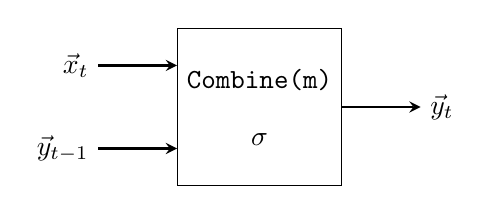
\begin{tikzpicture}
		\node[rectangle, draw, align=center, text depth=0em, minimum width=0.5cm,minimum height=2cm] (W1) {{\tt Combine(m)}\\[2ex]$\sigma$};
		\node[left=of W1, yshift=1.5em] (X) {$\vec{x}_t$};
		\node[left=of W1, yshift=-1.5em] (Y) {$\vec{y}_{t-1}$};
		\node[right=of W1] (Z) {$\vec{y}_t$};
		\draw[-stealth, thick] (X) -- ([yshift=1.5em]W1.west);
		\draw[-stealth, thick] (Y) -- ([yshift=-1.5em]W1.west);
		\draw[-stealth, thick] (W1) -- (Z);
		\end{tikzpicture}
	\end{center}
	Let's look into what we should choose for our SimpleRNN's $\sigma$\dots
\end{frame}

\begin{frame}
	\frametitle{SimpleRNN activations}
	\begin{itemize}
		\item \emph{Identity}: not useful (want to model \emph{nonlinear problems})\dots
		\vfill
		\item \emph{ReLU}: should be a natural first choice.\\BUT: \textbf{exploding gradients}!
		\vfill
		\item \emph{Sigmoid}: tanh preferred to the logistic function (for symmetry).\\BUT: \textbf{vanishing gradients}!
	\end{itemize}
\end{frame}

\begin{frame}
	\frametitle{A brief intro to gradient descent}
	\begin{itemize}
		\item Weights of a neural network are updated in the direction of the \emph{negative gradient} of the loss with respect to them:
		\[\vec{w}_t \leftarrow \vec{w}_{t-1} - \eta\nabla\mathcal{L}(\vec{w})\]
		where $\nabla\mathcal{L}(\vec{w}) = \begin{pmatrix}\frac{\partial\mathcal{L}(\vec{w})}{\partial w_1} & \dots & \frac{\partial\mathcal{L}(\vec{w})}{\partial w_n}\end{pmatrix}$
		\vfill
		\item Gradients are computed in an iterative fashion, starting from output neurons backwards to the inputs, using the \emph{chain rule}.
	\end{itemize}
\end{frame}

\begin{frame}
	\frametitle{A simple example}
	\begin{itemize}
		\item Consider a very simple ``path'' neural network, where each layer has only one neuron, each computing the same activation $\sigma$:
	\end{itemize}
	\vfill
	\begin{center}
		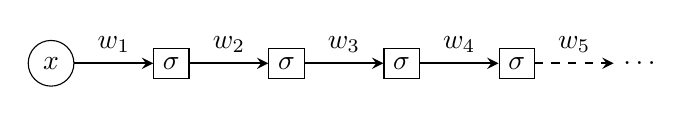
\begin{tikzpicture}
			\node[circle, draw] (X) {$x$};
			\node[rectangle, draw, right=of X] (A) {$\sigma$};
			\node[rectangle, draw, right=of A] (B) {$\sigma$};
			\node[rectangle, draw, right=of B] (C) {$\sigma$};
			\node[rectangle, draw, right=of C] (D) {$\sigma$};
			\node[rectangle, right=of D] (E) {\dots};
			\draw[-stealth, thick] (X) -- node[above] {$w_1$} (A);
			\draw[-stealth, thick] (A) -- node[above] {$w_2$} (B);
			\draw[-stealth, thick] (B) -- node[above] {$w_3$} (C);
			\draw[-stealth, thick] (C) -- node[above] {$w_4$} (D);
			\draw[-stealth, dashed, thick] (D) -- node[above] {$w_5$} (E);
		\end{tikzpicture}
	\end{center}
	\vfill
	\begin{itemize}
		\item Although this is a ``toy'' example, the conclusions will naturally carry over to wider networks (can be decomposed into many such paths, over which we ``accumulate'' gradient updates). 
		\vfill
		\item For a \emph{recurrent} neural network, these paths can grow at least as long as the number of steps in the input!
	\end{itemize}
\end{frame}

\begin{frame}
	\frametitle{Gradient updates}
	\begin{itemize}
	\item Let $a_i$ be the $i$-th neuron's activation, and $z_i$ be its output:\[z_0 = x,\ \ \ \ \ \ \ \ \ \ \ a_i = w_iz_{i-1},\ \ \ \ \ \ \ \ \ \ \ z_i = \sigma(a_i)\]
	\vfill
	\item Now, consider the partial derivative of the loss function with respect to $w_2$, by repeatedly applying the chain rule:
		\begin{align*}\frac{\partial\mathcal{L}(\vec{w})}{\partial w_2} &= \frac{\partial\mathcal{L}(\vec{w})}{\partial a_2}\frac{\partial a_2}{\partial w_2} = \sigma(a_1)\frac{\partial\mathcal{L}(\vec{w})}{\partial a_3}\frac{\partial a_3}{\partial z_2}\frac{\partial z_2}{\partial a_2}\\ &= \sigma(a_1)\sigma'(a_2)w_3\frac{\partial\mathcal{L}(\vec{w})}{\partial a_4}\frac{\partial a_4}{\partial z_3}\frac{\partial z_3}{\partial a_3}\\
			&= \sigma(a_1)\sigma'(a_2)w_3\sigma'(a_3)w_4\frac{\partial\mathcal{L}(\vec{w})}{\partial a_5}\frac{\partial a_5}{\partial z_4}\frac{\partial z_4}{\partial a_4}\\ &= \dots (\text{you see where this is going\dots})\\
			\end{align*}
	\end{itemize}
\end{frame}

\begin{frame}
	\frametitle{Vanishing gradients}
	\begin{itemize}
		\item In general, the gradient with respect to $w_2$ will be: 
		\[\sigma(a_1)\times \sigma'(a_2)\times w_3\times \sigma'(a_3)\times w_4\times \sigma'(a_4)\times \dots\]
		\vfill
		\item For RNNs applied to very long sequences, this product includes \emph{a lot} of $\sigma'$s when considering the first RNN block!
		\vfill
		\item When $\sigma$ is a sigmoid activation:
		\begin{itemize}
			\item Logistic: $\sigma'(x) = \sigma(x)(1 - \sigma(x)) \implies |\sigma'(x)| \leq 0.25$.
			\item tanh: $\sigma'(x) = 1 - \sigma(x)^2 \implies |\sigma'(x)| \leq 1$.
		\end{itemize}
		\vfill
		\item When you multiply many values with magnitudes less than one\dots the gradient \textbf{vanishes}!
	\end{itemize}
\end{frame}

\begin{frame}
	\frametitle{Exploding gradients}
	\begin{itemize}
		\item In general, the gradient with respect to $w_2$ will be: 
		\[\sigma(a_1)\times \sigma'(a_2)\times w_3\times \sigma'(a_3)\times w_4\times \sigma'(a_4)\times \dots\]
		\vfill
		\item ReLUs solve the vanishing gradient problem by having a derivative of $1$ when a neuron is ``alive'', and $0$ otherwise.
		\vfill
		\item However, the value of $\sigma(a_1)$ may grow without bound! 
		\vfill
		\item This is not overly troublesome for feedforward networks, but recurrent networks \emph{share weights}, so this update is applied once for each starting position.
		\vfill
		\item When you add up many updates that may grow without bound\dots the gradient easily \textbf{explodes}!
	\end{itemize}
\end{frame}

\begin{frame}
	\frametitle{Handling exploding gradients}
	\begin{itemize}
		\item To make exploding gradients manageable we apply \emph{gradient clipping}: making the gradient's norm no larger than a \emph{threshold}:
		\[\nabla\mathcal{L} = \nabla\mathcal{L}\frac{\nabla_{max}}{\max(||\nabla\mathcal{L}||, \nabla_{max})}\]
		\vfill
		\item While this is convenient, it will stop important \emph{long-term dependencies} from fully coming through---as was the case with vanishing gradients.
		\vfill
		\item Handling \emph{vanishing gradients} leads us to the central theme of this lecture\dots
	\end{itemize}
\end{frame}

\section{LSTM}

\begin{frame}
	\frametitle{Long Short-Term Memory}
	\begin{itemize}
		\item Proposed by Hochreiter and Schmidhuber (1997).
		\vfill
		\item Introduce a \emph{memory cell}, $\vec{c}$, which \emph{maintains features between time steps}, and explicitly control, based on the $\vec{x}_t$ and $\vec{y}_{t-1}$:
		\begin{itemize}
			\item What proportion of newly computed features \emph{enters} the cell;
			\item What proportion of the previously stored cell state is \emph{retained};
			\item What proportion of the new cell contents \emph{exits} the LSTM. 
		\end{itemize}
		\vfill
		\item This architecture \emph{solves} the vanishing gradient problem:
		\begin{itemize}
			\item We dynamically \emph{learn} the rate at which we want the gradient to vanish, with respect to the current inputs.
		\end{itemize}
	\end{itemize}
\end{frame}

\begin{frame}
	\frametitle{An LSTM block}
\makebox[\textwidth][c]{
	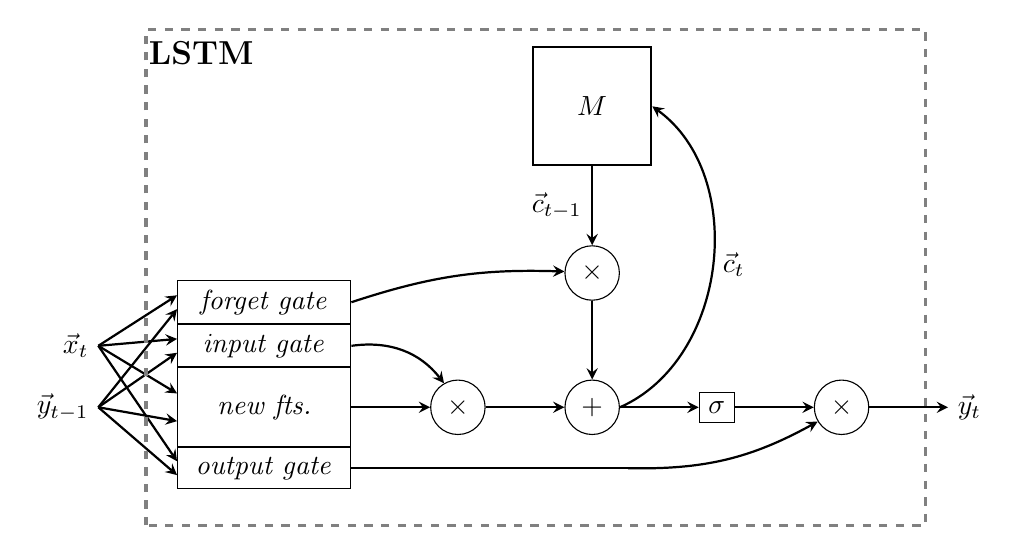
\begin{tikzpicture}
		
		\node[rectangle, draw, minimum width=2.2cm, minimum height=1cm] (FT) {\emph{new fts.}}; 
		\node[rectangle, above =0em of FT, draw, minimum width=2.2cm] (IG) {\emph{input gate}};
		\node[rectangle, above=0em of IG, draw, minimum width=2.2cm] (FG) {\emph{forget gate}};
		\node[rectangle, below=0em of FT, draw, minimum width=2.2cm] (OG) {\emph{output gate}};
		\node[left=of IG] (X) {$\vec{x}_t$};
		\node[left=of FT] (Y) {$\vec{y}_{t-1}$};
		
		\draw[-stealth, thick] (X.east) -- ([yshift=0.5em]FT.west);
		\draw[-stealth, thick] (X.east) -- ([yshift=0.25em]IG.west);
		\draw[-stealth, thick] (X.east) -- ([yshift=0.25em]FG.west);
		\draw[-stealth, thick] (X.east) -- ([yshift=0.25em]OG.west);
		\draw[-stealth, thick] (Y.east) -- ([yshift=-0.5em]FT.west);
		\draw[-stealth, thick] (Y.east) -- ([yshift=-0.25em]IG.west);
		\draw[-stealth, thick] (Y.east) -- ([yshift=-0.25em]FG.west);
		\draw[-stealth, thick] (Y.east) -- ([yshift=-0.25em]OG.west);
		
		\node[circle, draw, right=of FT] (t1) {$\times$};
		\node[circle, draw, right=of t1] (pl) {$+$};
		\node[rectangle, draw, right=of pl] (th) {$\sigma$};
		\node[circle, draw, right=of th] (t2) {$\times$};
		\node[right=of t2] (Y1) {$\vec{y}_t$};
		
		\node[circle, draw, above=of pl] (t3) {$\times$};
		
		\node[rectangle, thick, draw, above=of t3, minimum width=1.5cm, minimum height=1.5cm] (M) {$M$};
		
		\draw[-stealth, thick] (FT) -- (t1);
		\draw[-stealth, thick] (t1) -- (pl);
		\draw[-stealth, thick] (pl) -- (th);
		\draw[-stealth, thick] (th) -- (t2);
		\draw[-stealth, thick] (t2) -- (Y1);
		\draw[-stealth, thick] (M) -- node[left] {$\vec{c}_{t-1}$} (t3);
		\draw[-stealth, thick] (t3) -- (pl);
		\path[-stealth, thick] (IG.east) edge[bend left] (t1);
		\draw[thick] (OG.east) -- ([xshift=10em]OG.east);
		\path[-stealth, thick] (OG.east) -- ([xshift=10em]OG.east) edge[bend right=15] (t2);
		\path[-stealth, thick] (FG.east) edge[bend left=10] (t3);
		\path[-stealth, thick] (pl.east) edge[bend right=60] node[right] {$\vec{c}_t$} (M.east);
		
		\draw[-stealth, very thick, dashed, gray] (-1.5, -1.5) rectangle (8.4, 4.8);
		\node[] (tttxt) at (-0.8, 4.5) {\large \bf LSTM};
	\end{tikzpicture}}
\end{frame}

\begin{frame}
	\frametitle{The \emph{``new features''} block}
	\begin{itemize}
		\item Compute the new features based on $\vec{x}_t$ and $\vec{y}_{t-1}$---essentially a SimpleRNN/``combine'' block!
		\vfill
		\item Since the LSTMs are designed to handle vanishing gradients, best to use the more stable sigmoid (\emph{tanh}) as the activation.
		\vfill
		\begin{center}
		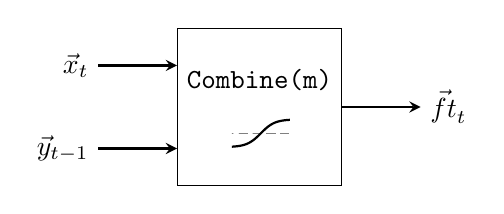
\begin{tikzpicture}
		\node[rectangle, draw, align=center, text depth=0em, minimum width=0.5cm,minimum height=2cm] (W1) {{\tt Combine(m)}\\[2ex]};
		%\node[rectangle, draw] (P1) {{
		\begin{axis}[xshift=-1em,yshift=-1.5em,
			samples=1000, domain=-2.6:2.6,
				hide axis,
				xtick=\empty,
				ytick=\empty,
				xlabel=\empty,
				ylabel=\empty,
				xmin=-2.1, xmax=2.1,
				ymin=-1.1, ymax=1.1,
				x=0.5em, y=0.5em,
				trig format = rad
			]
				\addplot expression [no markers, smooth, densely dashed, gray] {0};
				\addplot expression [no markers, smooth, thick, black] {tanh(\x)};
			\end{axis}%}};
		\node[left=of W1, yshift=1.5em] (X) {$\vec{x}_t$};
		\node[left=of W1, yshift=-1.5em] (Y) {$\vec{y}_{t-1}$};
		\node[right=of W1] (Z) {$\vec{ft}_t$};
		\draw[-stealth, thick] (X) -- ([yshift=1.5em]W1.west);
		\draw[-stealth, thick] (Y) -- ([yshift=-1.5em]W1.west);
		\draw[-stealth, thick] (W1) -- (Z);
		\end{tikzpicture}
	\end{center}
	\vfill
	\[\vec{ft}_t = \tanh\left({\bf W}_{ft}\vec{x}_t + {\bf U}_{ft}\vec{y}_{t-1} + \vec{b}_{ft}\right)\]
	\vfill
	\item Similarly, we should use tanh as the output activation ($\sigma$).
	\end{itemize}
\end{frame}

\begin{frame}
	\frametitle{The input/output/forget gates}
	\begin{itemize}
		\item Compute the required proportions based on $\vec{x}_t$ and $\vec{y}_{t-1}$---yet another ``combine'' block!
		\vfill
		\item Want a value in the [0, 1] range per feature (0/1--block/pass completely), so the \emph{logistic} sigmoid is appropriate here.
		\vfill
		\begin{center}
		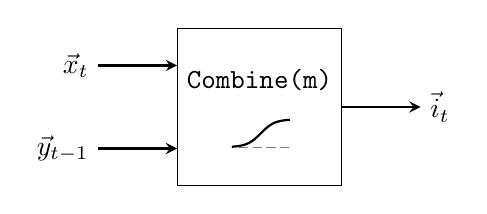
\begin{tikzpicture}
		\node[rectangle, draw, align=center, text depth=0em, minimum width=0.5cm,minimum height=2cm] (W1) {{\tt Combine(m)}\\[2ex]};
		%\node[rectangle, draw] (P1) {{
		\begin{axis}[xshift=-1em,yshift=-1.5em,
			samples=1000, domain=-2.6:2.6,
				hide axis,
				xtick=\empty,
				ytick=\empty,
				xlabel=\empty,
				ylabel=\empty,
				xmin=-2.1, xmax=2.1,
				ymin=-1.1, ymax=1.1,
				x=0.5em, y=0.5em,
				trig format = rad
			]
				\addplot expression [no markers, smooth, densely dashed, gray] {-1};
				\addplot expression [no markers, smooth, thick, black] {tanh(\x)};
			\end{axis}%}};
		\node[left=of W1, yshift=1.5em] (X) {$\vec{x}_t$};
		\node[left=of W1, yshift=-1.5em] (Y) {$\vec{y}_{t-1}$};
		\node[right=of W1] (Z) {$\vec{i}_t$};
		\draw[-stealth, thick] (X) -- ([yshift=1.5em]W1.west);
		\draw[-stealth, thick] (Y) -- ([yshift=-1.5em]W1.west);
		\draw[-stealth, thick] (W1) -- (Z);
		\end{tikzpicture}
	\end{center}
	\vfill
	\[\vec{i}_t = logistic\left({\bf W}_{i}\vec{x}_t + {\bf U}_{i}\vec{y}_{t-1} + \vec{b}_{i}\right)\]
	\vfill
	\item (Similarly for $\vec{o}_t$ and $\vec{f}_t$\dots)
	\end{itemize}
\end{frame}

\begin{frame}
	\frametitle{Putting it all together}
	\begin{align*}\vec{i}_t &= logistic\left({\bf W}_{i}\vec{x}_t + {\bf U}_{i}\vec{y}_{t-1} + \vec{b}_{i}\right)\tikzmark{gstart}\\	
	\vec{f}_t &= logistic\left({\bf W}_{f}\vec{x}_t + {\bf U}_{f}\vec{y}_{t-1} + \vec{b}_{f}\right)\\
	\vec{o}_t &= logistic\left({\bf W}_{o}\vec{x}_t + {\bf U}_{o}\vec{y}_{t-1} + \vec{b}_{o}\right)\tikzmark{gend}\\
	\vec{ft}_t &= \tanh\left({\bf W}_{ft}\vec{x}_t + {\bf U}_{ft}\vec{y}_{t-1} + \vec{b}_{ft}\right) \tikzmark{fst}\\
	\vec{c}_t &= \vec{ft}_t \otimes \vec{i}_t + \vec{c}_{t-1} \otimes \vec{f}_t \tikzmark{ust}\\
	\vec{y}_t &= \tanh\left(\vec{c}_t\right) \otimes \vec{o}_t \tikzmark{ost}\end{align*}
	
	\begin{tikzpicture}[overlay, remember picture]
\draw [decoration={brace,amplitude=0.4em},decorate,ultra thick]
([yshift=5.8em]gend.south east) -- node[right=0.5em] {\emph{gates}} ([yshift=-0.4em]gend.south east);
\draw [decoration={brace,amplitude=0.4em},decorate,ultra thick]
([yshift=1.5em]fst.south east) -- node[right=0.5em] {\emph{new features}} ([yshift=-0.3em]fst.south east);
\draw [decoration={brace,amplitude=0.4em},decorate,ultra thick]
([yshift=1.4em]ust.south east) -- node[right=0.5em] {\emph{update cell}} ([yshift=-0.2em]ust.south east);
\draw [decoration={brace,amplitude=0.4em},decorate,ultra thick]
([yshift=1.4em]ost.south east) -- node[right=0.5em] {\emph{output}} ([yshift=-0.2em]ost.south east);
\end{tikzpicture}
\end{frame}

\begin{frame}
	\frametitle{Creating \emph{deep} LSTMs}
	\makebox[\textwidth][c]{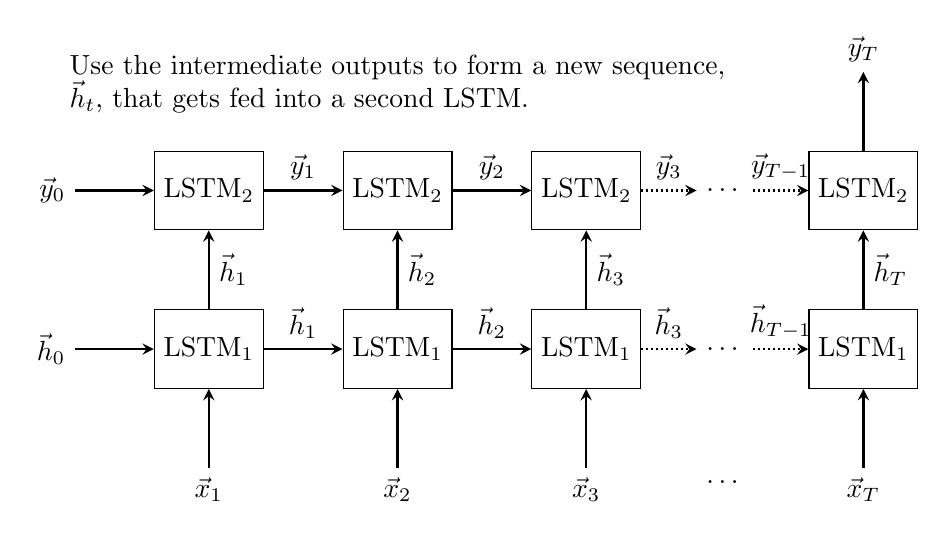
\begin{tikzpicture}
			\node[rectangle, draw, minimum height=1cm, minimum width=1cm] (RNN) at (0, 0) {LSTM$_1$};
			\node[rectangle, right=of RNN, draw, minimum height=1cm, minimum width=1cm] (RNN2) {LSTM$_1$};
			\node[rectangle, right=of RNN2, draw, minimum height=1cm, minimum width=1cm] (RNN3) {LSTM$_1$};
			
			\node[rectangle, right=2em of RNN3] (RNN4) {\dots};
			\node[rectangle, right=2em of RNN4, draw, minimum height=1cm, minimum width=1cm] (RNN5) {LSTM$_1$};
			
			\node[rectangle, draw, above=of RNN, minimum height=1cm, minimum width=1cm] (R21) {LSTM$_2$};
			\node[rectangle, right=of R21, draw, minimum height=1cm, minimum width=1cm] (R22) {LSTM$_2$};
			\node[rectangle, right=of R22, draw, minimum height=1cm, minimum width=1cm] (R23) {LSTM$_2$};
			
			\node[rectangle, right=2em of R23] (R24) {\dots};
			\node[rectangle, right=2em of R24, draw, minimum height=1cm, minimum width=1cm] (R25) {LSTM$_2$};
			
			\node[above=1em of R22, align=left] {
	Use the intermediate outputs to form a new sequence,\\ $\vec{h}_t$, that gets fed into a second LSTM.};
			
			\node[below=of RNN] (X1) {$\vec{x}_1$};
			\node[below=of RNN2] (X2) {$\vec{x}_2$};
			\node[below=of RNN3] (X3) {$\vec{x}_3$};
			\node[below=of RNN5] (X4) {$\vec{x}_T$};
			\node[above=of R25] (Y) {$\vec{y}_T$};
			\node[left=of RNN] (Y0) {$\vec{h}_0$};
			\node[left=of R21] (Y20) {$\vec{y}_0$};
			
			\draw[-stealth, thick] (X1) -- (RNN);
			\draw[-stealth, thick] (X2) -- (RNN2);
			\draw[-stealth, thick] (X3) -- (RNN3);
			\draw[-stealth, thick] (X4) -- (RNN5);
			\draw[-stealth, thick] (Y0) -- (RNN);
			\draw[-stealth, thick] (R25) -- (Y);
			\draw[-stealth, thick] (RNN) -- node[above] {$\vec{h}_1$} (RNN2);
			\draw[-stealth, thick] (RNN2) -- node[above] {$\vec{h}_2$} (RNN3);
			\draw[-stealth, densely dotted, thick] (RNN3) -- node[above] {$\vec{h}_3$} (RNN4);
			\draw[-stealth, densely dotted, thick] (RNN4) -- node[above] {$\vec{h}_{T-1}$} (RNN5);
			\node[below=4em of RNN4] (d) {\dots};
			
			\draw[-stealth, thick] (RNN) -- node[right] {$\vec{h}_1$} (R21);
			\draw[-stealth, thick] (RNN2) -- node[right] {$\vec{h}_2$} (R22);
			\draw[-stealth, thick] (RNN3) -- node[right] {$\vec{h}_3$} (R23);
			\draw[-stealth, thick] (RNN5) -- node[right] {$\vec{h}_T$} (R25);
			\draw[-stealth, thick] (Y20) -- (R21);
			
			
			\draw[-stealth, thick] (R21) -- node[above] {$\vec{y}_1$} (R22);
			\draw[-stealth, thick] (R22) -- node[above] {$\vec{y}_2$} (R23);
			\draw[-stealth, densely dotted, thick] (R23) -- node[above] {$\vec{y}_3$} (R24);
			\draw[-stealth, densely dotted, thick] (R24) -- node[above] {$\vec{y}_{T-1}$} (R25);
			
		\end{tikzpicture}}
\end{frame}

\begin{frame}
	\frametitle{Tips `n' Tricks: Initialisation and optimisers}
	\begin{itemize}
		\item It is important to choose the initial parameter values to help the LSTM learn effectively in the early stages!
		\vfill
		\item Sensible initialisations are (Keras does these \emph{automatically}):
		\begin{itemize}
			\item ${\bf U}_*$ as \emph{orthonormal} matrices (help combat vanishing gradients even further; eigenvalues $\sim$ 1).
			\item $\vec{b}_f = \vec{1}$ (to encourage long-term dependencies early on); 
			\item \emph{Xavier initialisation} (Glorot and Bengio (2010)) for all other weights (\emph{recommended} for sigmoid activations).
		\end{itemize}
		\vfill
		\item Gradient descent algorithms that automatically tune the learning rate are now common---for RNNs, \emph{Adam} (Kingma and Ba (2014)) and \emph{RMSProp} (Tieleman and Hinton (2012)) work particularly well.
	\end{itemize}
\end{frame}

\begin{frame}
	\frametitle{Tips `n' Tricks: Dropout}
	\begin{itemize}
		\item Randomly ``kill'' neurons \emph{during training only}.\\ (Srivastava et al. (2014))
	\end{itemize}
	\vfill
	\begin{center}
	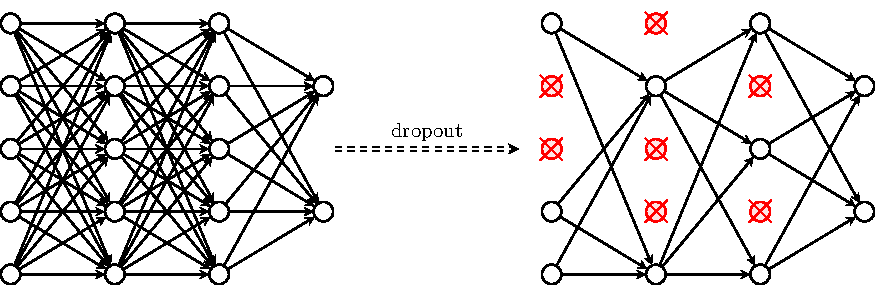
\includegraphics[width=1.0\linewidth]{dropout.pdf}
	\end{center}
	\vfill
	\begin{itemize}
		\item Forces network to \emph{not rely} on existence of some neuron\dots
	\end{itemize}
\end{frame}


\begin{frame}
	\frametitle{Tips `n' Tricks: Dropout in LSTMs}
	\makebox[\textwidth][c]{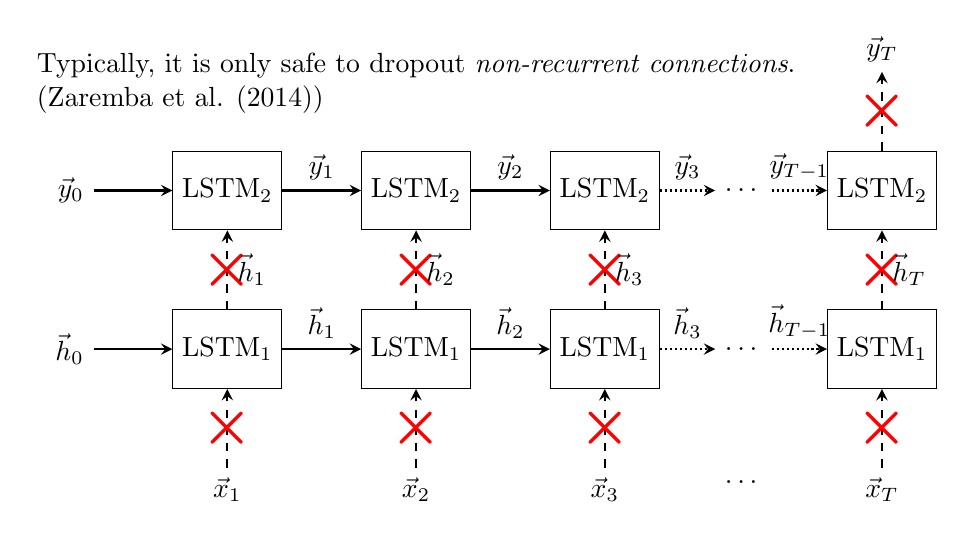
\begin{tikzpicture}
			\node[rectangle, draw, minimum height=1cm, minimum width=1cm] (RNN) at (0, 0) {LSTM$_1$};
			\node[rectangle, right=of RNN, draw, minimum height=1cm, minimum width=1cm] (RNN2) {LSTM$_1$};
			\node[rectangle, right=of RNN2, draw, minimum height=1cm, minimum width=1cm] (RNN3) {LSTM$_1$};
			
			\node[rectangle, right=2em of RNN3] (RNN4) {\dots};
			\node[rectangle, right=2em of RNN4, draw, minimum height=1cm, minimum width=1cm] (RNN5) {LSTM$_1$};
			
			\node[rectangle, draw, above=of RNN, minimum height=1cm, minimum width=1cm] (R21) {LSTM$_2$};
			\node[rectangle, right=of R21, draw, minimum height=1cm, minimum width=1cm] (R22) {LSTM$_2$};
			\node[rectangle, right=of R22, draw, minimum height=1cm, minimum width=1cm] (R23) {LSTM$_2$};
			
			\node[rectangle, right=2em of R23] (R24) {\dots};
			\node[rectangle, right=2em of R24, draw, minimum height=1cm, minimum width=1cm] (R25) {LSTM$_2$};
			
			\node[above=1em of R22, align=left] {
	Typically, it is only safe to dropout \emph{non-recurrent connections}.\\(Zaremba et al. (2014))};
			
			\node[below=of RNN] (X1) {$\vec{x}_1$};
			\node[below=of RNN2] (X2) {$\vec{x}_2$};
			\node[below=of RNN3] (X3) {$\vec{x}_3$};
			\node[below=of RNN5] (X4) {$\vec{x}_T$};
			\node[above=of R25] (Y) {$\vec{y}_T$};
			\node[left=of RNN] (Y0) {$\vec{h}_0$};
			\node[left=of R21] (Y20) {$\vec{y}_0$};
			
			\draw[-stealth, thick, dashed] (X1) -- node[midway, red] {$\mathlarger{\mathlarger{\mathlarger{\mathlarger{\mathlarger{\bm{\times}}}}}}$} (RNN);
			\draw[-stealth, thick, dashed] (X2) -- node[midway, red] {$\mathlarger{\mathlarger{\mathlarger{\mathlarger{\mathlarger{\bm{\times}}}}}}$} (RNN2);
			\draw[-stealth, thick, dashed] (X3) -- node[midway, red] {$\mathlarger{\mathlarger{\mathlarger{\mathlarger{\mathlarger{\bm{\times}}}}}}$} (RNN3);
			\draw[-stealth, thick, dashed] (X4) -- node[midway, red] {$\mathlarger{\mathlarger{\mathlarger{\mathlarger{\mathlarger{\bm{\times}}}}}}$} (RNN5);
			\draw[-stealth, thick] (Y0) -- (RNN);
			\draw[-stealth, dashed, thick] (R25) -- node[midway, red] {$\mathlarger{\mathlarger{\mathlarger{\mathlarger{\mathlarger{\bm{\times}}}}}}$} (Y);
			\draw[-stealth, thick] (RNN) -- node[above] {$\vec{h}_1$} (RNN2);
			\draw[-stealth, thick] (RNN2) -- node[above] {$\vec{h}_2$} (RNN3);
			\draw[-stealth, densely dotted, thick] (RNN3) -- node[above] {$\vec{h}_3$} (RNN4);
			\draw[-stealth, densely dotted, thick] (RNN4) -- node[above] {$\vec{h}_{T-1}$} (RNN5);
			\node[below=4em of RNN4] (d) {\dots};
			
			\draw[-stealth, dashed, thick] (RNN) -- node[midway, red] {$\mathlarger{\mathlarger{\mathlarger{\mathlarger{\mathlarger{\bm{\times}}}}}}$} node[right] {$\vec{h}_1$} (R21);
			\draw[-stealth,dashed, thick] (RNN2) -- node[midway, red] {$\mathlarger{\mathlarger{\mathlarger{\mathlarger{\mathlarger{\bm{\times}}}}}}$} node[right] {$\vec{h}_2$} (R22);
			\draw[-stealth,dashed, thick] (RNN3) -- node[midway, red] {$\mathlarger{\mathlarger{\mathlarger{\mathlarger{\mathlarger{\bm{\times}}}}}}$} node[right] {$\vec{h}_3$} (R23);
			\draw[-stealth,dashed, thick] (RNN5) -- node[midway, red] {$\mathlarger{\mathlarger{\mathlarger{\mathlarger{\mathlarger{\bm{\times}}}}}}$} node[right] {$\vec{h}_T$} (R25);
			\draw[-stealth, thick] (Y20) -- (R21);
			
			
			\draw[-stealth, thick] (R21) -- node[above] {$\vec{y}_1$} (R22);
			\draw[-stealth, thick] (R22) -- node[above] {$\vec{y}_2$} (R23);
			\draw[-stealth, densely dotted, thick] (R23) -- node[above] {$\vec{y}_3$} (R24);
			\draw[-stealth, densely dotted, thick] (R24) -- node[above] {$\vec{y}_{T-1}$} (R25);
			
		\end{tikzpicture}}
\end{frame}

\begin{frame}
	\frametitle{Tips `n' Tricks: Bidirectional LSTM}
	\begin{itemize}
		\item Very often, the dependencies within sequential data are not just in \emph{one} direction, but may be observed in \emph{both}!
		\vfill
		\item Examples: DNA strands, words in a sentence, \dots
		\vfill
		\item Bidirectional layers exploit this by combining the features obtained going in both directions simultaneously.
		\vfill
		\item Very simple to deploy in Keras ({\tt Bidirectional} wrapper around recurrent layers).
	\end{itemize}
\end{frame}

\begin{frame}
	\frametitle{Tips `n' Tricks: Bidirectional LSTM in action}
	\makebox[\textwidth][c]{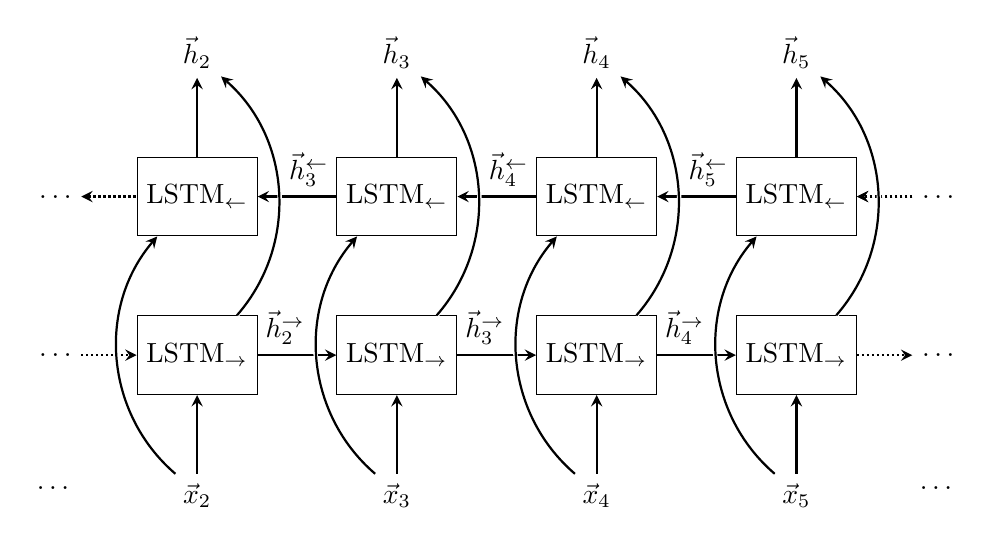
\begin{tikzpicture}
			\node[rectangle] (Y0) at (0, 0) {$\dots$};
			\node[rectangle, draw, right=2em of Y0, minimum height=1cm, minimum width=1cm] (RNN) {LSTM$_\rightarrow$};
			\node[rectangle, right=of RNN, draw, minimum height=1cm, minimum width=1cm] (RNN2) {LSTM$_\rightarrow$};
			\node[rectangle, right=of RNN2, draw, minimum height=1cm, minimum width=1cm] (RNN3) {LSTM$_\rightarrow$};
			
			\node[rectangle, right= of RNN3, draw, minimum height=1cm, minimum width=1cm] (RNN4) {LSTM$_\rightarrow$};
			\node[rectangle, right=2em of RNN4] (RNN5) {$\dots$};
			
			
			\node[rectangle, above=of RNN4, draw, minimum height=1cm, minimum width=1cm] (R25) {LSTM$_\leftarrow$};
			\node[rectangle, left=of R25, minimum height=1cm, minimum width=1cm, draw] (R24) {LSTM$_\leftarrow$};
			\node[rectangle, left=of R24, draw, minimum height=1cm, minimum width=1cm] (R23) {LSTM$_\leftarrow$};
			\node[rectangle, left=of R23, draw, minimum height=1cm, minimum width=1cm] (R22) {LSTM$_\leftarrow$};
			\node[rectangle, left=2em of R22] (R21) {$\dots$};
			\node[right=2em of R25] (Y20) {$\dots$};
			
			
			%\node[above=1em of R22, align=left] {
	%Process input sequence in \emph{both directions}, when appropriate.};
			
			\node[below=of RNN] (X1) {$\vec{x}_2$};
			\node[below=of RNN2] (X2) {$\vec{x}_3$};
			\node[below=of RNN3] (X3) {$\vec{x}_4$};
			\node[below=of RNN4] (X4) {$\vec{x}_5$};
			\node[above=of R25] (Y5) {$\vec{h}_5$};
			\node[above=of R24] (Y4) {$\vec{h}_4$};
			\node[above=of R23] (Y3) {$\vec{h}_3$};
			\node[above=of R22] (Y2) {$\vec{h}_2$};
			
			\draw[-stealth, thick] (X1) -- (RNN);
			\draw[-stealth, thick] (X2) -- (RNN2);
			\draw[-stealth, thick] (X3) -- (RNN3);
			\draw[-stealth, thick] (X4) -- (RNN4);
			\draw[-stealth, thick, densely dotted] (Y0) -- (RNN);
			\draw[-stealth, thick] (RNN) -- node[above, pos=0.35] {$\vec{h}_2^\rightarrow$} (RNN2);
			\draw[-stealth, thick] (RNN2) -- node[above, pos=0.35] {$\vec{h}_3^\rightarrow$} (RNN3);
			\draw[-stealth, thick] (RNN3) -- node[above, pos=0.35] {$\vec{h}_4^\rightarrow$} (RNN4);
			\draw[-stealth, densely dotted, thick] (RNN4) -- (RNN5);
			\node[below=4em of Y0] (d) {\dots};
			\node[below=4em of RNN5] (d) {\dots};
			
			\path[-stealth, ultra thick, white] (X1) edge[bend left=45] (R22);
			\path[-stealth, thick] (X1) edge[bend left=45] (R22);
			\path[-stealth, ultra thick, white] (X2) edge[bend left=45] (R23);
			\path[-stealth, thick] (X2) edge[bend left=45] (R23);
			\path[-stealth, ultra thick, white] (X3) edge[bend left=45] (R24);
			\path[-stealth, thick] (X3) edge[bend left=45] (R24);
			\path[-stealth, ultra thick, white] (X4) edge[bend left=45] (R25);
			\path[-stealth, thick] (X4) edge[bend left=45] (R25);
			\draw[-stealth, densely dotted, thick] (Y20) -- (R25);
			
			\draw[-stealth, thick] (R22) -- (Y2);
			\draw[-stealth, thick] (R23) -- (Y3);
			\draw[-stealth, thick] (R24) -- (Y4);
			\draw[-stealth, thick] (R25) -- (Y5);
			
			
			\draw[stealth-, densely dotted, thick] (R21) -- (R22);
			\draw[stealth-, thick] (R22) -- node[above, pos=0.65] {$\vec{h}_3^\leftarrow$} (R23);
			\draw[stealth-, thick] (R23) -- node[above, pos=0.65] {$\vec{h}_4^\leftarrow$} (R24);
			\draw[stealth-, thick] (R24) -- node[above, pos=0.65] {$\vec{h}_5^\leftarrow$} (R25);
			\draw[-stealth, densely dotted, thick] (Y20) -- (R25);
			
			
			\path[-stealth, ultra thick, white] (RNN) edge[bend right=45] (Y2);
			\path[-stealth, thick] (RNN) edge[bend right=45] (Y2);
			\path[-stealth, ultra thick, white] (RNN2) edge[bend right=45] (Y3);
			\path[-stealth, thick] (RNN2) edge[bend right=45] (Y3);
			\path[-stealth, ultra thick, white] (RNN3) edge[bend right=45] (Y4);
			\path[-stealth, thick] (RNN3) edge[bend right=45] (Y4);
			\path[-stealth, ultra thick, white] (RNN4) edge[bend right=45] (Y5);
			\path[-stealth, thick] (RNN4) edge[bend right=45] (Y5);
			
		\end{tikzpicture}}
\end{frame}

\begin{frame}
	\frametitle{\emph{Demo:} The \emph{Josef K.} LSTM}
	\begin{itemize}
		\item \emph{Character-level} language model: based on the previous $n$ characters observed in a text, predict the next one.
		\vfill
		\item Two-layer LSTM (with 512 features in each layer), trained on Franz Kafka's \emph{The Trial} (\emph{Der Prozess}):\\
		{\tt inp = Input(shape=(seq\_len, vocab\_len))\\
		h\_1 = LSTM(512, return\_sequences=True)(inp)\\
		h\_2 = LSTM(512, dropout\_W=0.5)(h\_1)\\
		out = Dense(vocab\_len, activation='softmax')(h\_2)} 
		\vfill
		\item Once trained, we can repeatedly sample the obtained probability distribution to \emph{generate our own text, one character at a time}!
	\end{itemize}
\end{frame}

\begin{frame}
	\frametitle{\emph{Demo:} Samples from the Josef K. LSTM\dots}
	{\tt "I'm not sure that's
worrible?" asked K.  "Yes," said the businessman, "and that's what they could do," said K., and was able to make things some place and he would need to be able to deal with the court which were the old man with a sigh for in the hallway which was already for him to de and darkness without being didned the bed.  "I'm sure this court would have been meant to be a little while to him in the court.  They were all asside the painter and looked at her with some way on his way and leave.  "It's nothing about your face when I had been given the first attention foreary, there was a lithle like that are not the time he remained standing with his head so far from the bank.}
\end{frame}

\begin{frame}
	\frametitle{Taking the idea further}
	\begin{itemize}
		\item The idea of repeatedly sampling the LSTM output and feeding it back to the input is a common one. For example, we might learn a classifier to predict a \emph{translation} of a given sentence, word by word.
		\vfill
		\item Or, if we feed in features extracted from an image (e.g. by using a convolutional neural network)\dots
	\end{itemize}
\end{frame}

\begin{frame}
	\frametitle{Neural Talk}
	\begin{itemize}
		\item Vinyals et al. (2014), Karpathy and Fei-Fei (2015).
	\end{itemize}
	\centering
	
\includegraphics[width=0.8\linewidth]{neural_talk.jpg}
\end{frame}

\begin{frame}
	\frametitle{Future prospects\dots}
	\begin{itemize}
		\item Although it seems like recurrent networks are the \emph{de facto} standard for processing sequential data, this may well change in the future.
		\vfill
		\item Feedforward models are \emph{significantly} easier to train, control and parallelise (fewer interdependencies).
		\vfill
		\item Recent work using \emph{\`{a} trous} (\emph{dilated}) convolutions on machine translation (Kalchbrenner et al. (2016)) and WaveNets (van den Oord et al. (2016)) outperforms or matches recurrent models in domains where they historically dominated.
	\end{itemize}
\end{frame}

\begin{frame}
	\frametitle{Regular $1\times 3$ convolution in 1D ({\tt Convolution1D})}	
	\begin{center}
	\begin{turn}{90}
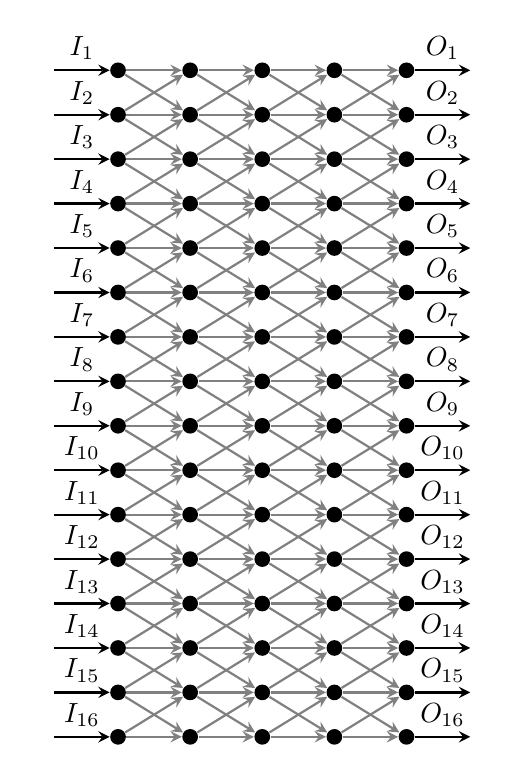
\begin{tikzpicture}[transform shape]
		\node[circle, fill, inner sep=0.2em] (s1) {};
		\node[circle, below=1em of s1, fill, inner sep=0.2em] (s2) {};
		\node[circle, below=1em of s2, fill, inner sep=0.2em] (s3) {};
		\node[circle, below=1em of s3, fill, inner sep=0.2em] (s4) {};
		\node[circle, below=1em of s4, fill, inner sep=0.2em] (s5) {};
		\node[circle, below=1em of s5, fill, inner sep=0.2em] (s6) {};
		\node[circle, below=1em of s6, fill, inner sep=0.2em] (s7) {};
		\node[circle, below=1em of s7, fill, inner sep=0.2em] (s8) {};
		\node[circle, below=1em of s8, fill, inner sep=0.2em] (s9) {};
		\node[circle, below=1em of s9, fill, inner sep=0.2em] (s10) {};
		\node[circle, below=1em of s10, fill, inner sep=0.2em] (s11) {};
		\node[circle, below=1em of s11, fill, inner sep=0.2em] (s12) {};
		\node[circle, below=1em of s12, fill, inner sep=0.2em] (s13) {};
		\node[circle, below=1em of s13, fill, inner sep=0.2em] (s14) {};
		\node[circle,below=1em of s14,  fill, inner sep=0.2em] (s15) {};
		\node[circle, below=1em of s15, fill, inner sep=0.2em] (s16) {};
		
		\foreach \x in {1,...,16}
    		\node[circle, right=2em of s\x, fill, inner sep=0.2em] (h\x) {};
		\foreach \x in {1,...,16}
    		\node[circle, right=2em of h\x, fill, inner sep=0.2em] (hh\x) {};
		\foreach \x in {1,...,16}
    		\node[circle, right=2em of hh\x, fill, inner sep=0.2em] (hhh\x) {};
		\foreach \x in {1,...,16}
    		\node[circle, right=2em of hhh\x, fill, inner sep=0.2em] (hhhh\x) {};
		\foreach \x in {1,...,16}
    		\node[circle, right=2em of hhhh\x] (o\x) {};
		\foreach \x in {1,...,16}
    		\node[circle, left=2em of s\x] (i\x) {};
    		
		\foreach \x in {1,...,16}
    		\draw[-stealth, thick] (i\x) --node[above] {$I_{\x}$} (s\x);
		\foreach \x in {1,...,16}
    		\draw[-stealth, thick] (hhhh\x) --node[above] {$O_{\x}$} (o\x);
		\foreach \x in {1,...,16}
    		\draw[-stealth, thick, gray] (s\x) -- (h\x);
		\foreach \x in {1,...,16}
    		\draw[-stealth, thick, gray] (h\x) -- (hh\x);
		\foreach \x in {1,...,16}
    		\draw[-stealth, thick, gray] (hh\x) -- (hhh\x);
		\foreach \x in {1,...,16}
    		\draw[-stealth, thick, gray] (hhh\x) -- (hhhh\x);
    		
    	\draw[-stealth, thick, gray] (s1) -- (h2);
    	\draw[-stealth, thick, gray] (s2) -- (h1);
    	\draw[-stealth, thick, gray] (s2) -- (h3);
    	\draw[-stealth, thick, gray] (s3) -- (h2);
    	\draw[-stealth, thick, gray] (s3) -- (h4);
    	\draw[-stealth, thick, gray] (s4) -- (h3);
    	\draw[-stealth, thick, gray] (s4) -- (h5);
    	\draw[-stealth, thick, gray] (s5) -- (h4);
    	\draw[-stealth, thick, gray] (s5) -- (h6);
    	\draw[-stealth, thick, gray] (s6) -- (h5);
    	\draw[-stealth, thick, gray] (s6) -- (h7);
    	\draw[-stealth, thick, gray] (s7) -- (h6);
    	\draw[-stealth, thick, gray] (s7) -- (h8);
    	\draw[-stealth, thick, gray] (s8) -- (h7);
    	\draw[-stealth, thick, gray] (s8) -- (h9);
    	\draw[-stealth, thick, gray] (s9) -- (h8);
    	\draw[-stealth, thick, gray] (s9) -- (h10);
    	\draw[-stealth, thick, gray] (s10) -- (h9);
    	\draw[-stealth, thick, gray] (s10) -- (h11);
    	\draw[-stealth, thick, gray] (s11) -- (h10);
    	\draw[-stealth, thick, gray] (s11) -- (h12);
    	\draw[-stealth, thick, gray] (s12) -- (h11);
    	\draw[-stealth, thick, gray] (s12) -- (h13);
    	\draw[-stealth, thick, gray] (s13) -- (h12);
    	\draw[-stealth, thick, gray] (s13) -- (h14);
    	\draw[-stealth, thick, gray] (s14) -- (h13);
    	\draw[-stealth, thick, gray] (s14) -- (h15);
    	\draw[-stealth, thick, gray] (s15) -- (h14);
    	\draw[-stealth, thick, gray] (s15) -- (h16);
    	\draw[-stealth, thick, gray] (s16) -- (h15);
    	
    	\draw[-stealth, thick, gray] (h1) -- (hh2);
    	\draw[-stealth, thick, gray] (h2) -- (hh1);
    	\draw[-stealth, thick, gray] (h2) -- (hh3);
    	\draw[-stealth, thick, gray] (h3) -- (hh2);
    	\draw[-stealth, thick, gray] (h3) -- (hh4);
    	\draw[-stealth, thick, gray] (h4) -- (hh3);
    	\draw[-stealth, thick, gray] (h4) -- (hh5);
    	\draw[-stealth, thick, gray] (h5) -- (hh4);
    	\draw[-stealth, thick, gray] (h5) -- (hh6);
    	\draw[-stealth, thick, gray] (h6) -- (hh5);
    	\draw[-stealth, thick, gray] (h6) -- (hh7);
    	\draw[-stealth, thick, gray] (h7) -- (hh6);
    	\draw[-stealth, thick, gray] (h7) -- (hh8);
    	\draw[-stealth, thick, gray] (h8) -- (hh7);
    	\draw[-stealth, thick, gray] (h8) -- (hh9);
    	\draw[-stealth, thick, gray] (h9) -- (hh8);
    	\draw[-stealth, thick, gray] (h9) -- (hh10);
    	\draw[-stealth, thick, gray] (h10) -- (hh9);
    	\draw[-stealth, thick, gray] (h10) -- (hh11);
    	\draw[-stealth, thick, gray] (h11) -- (hh10);
    	\draw[-stealth, thick, gray] (h11) -- (hh12);
    	\draw[-stealth, thick, gray] (h12) -- (hh11);
    	\draw[-stealth, thick, gray] (h12) -- (hh13);
    	\draw[-stealth, thick, gray] (h13) -- (hh12);
    	\draw[-stealth, thick, gray] (h13) -- (hh14);
    	\draw[-stealth, thick, gray] (h14) -- (hh13);
    	\draw[-stealth, thick, gray] (h14) -- (hh15);
    	\draw[-stealth, thick, gray] (h15) -- (hh14);
    	\draw[-stealth, thick, gray] (h15) -- (hh16);
    	\draw[-stealth, thick, gray] (h16) -- (hh15);
    	
    	\draw[-stealth, thick, gray] (hh1) -- (hhh2);
    	\draw[-stealth, thick, gray] (hh2) -- (hhh1);
    	\draw[-stealth, thick, gray] (hh2) -- (hhh3);
    	\draw[-stealth, thick, gray] (hh3) -- (hhh2);
    	\draw[-stealth, thick, gray] (hh3) -- (hhh4);
    	\draw[-stealth, thick, gray] (hh4) -- (hhh3);
    	\draw[-stealth, thick, gray] (hh4) -- (hhh5);
    	\draw[-stealth, thick, gray] (hh5) -- (hhh4);
    	\draw[-stealth, thick, gray] (hh5) -- (hhh6);
    	\draw[-stealth, thick, gray] (hh6) -- (hhh5);
    	\draw[-stealth, thick, gray] (hh6) -- (hhh7);
    	\draw[-stealth, thick, gray] (hh7) -- (hhh6);
    	\draw[-stealth, thick, gray] (hh7) -- (hhh8);
    	\draw[-stealth, thick, gray] (hh8) -- (hhh7);
    	\draw[-stealth, thick, gray] (hh8) -- (hhh9);
    	\draw[-stealth, thick, gray] (hh9) -- (hhh8);
    	\draw[-stealth, thick, gray] (hh9) -- (hhh10);
    	\draw[-stealth, thick, gray] (hh10) -- (hhh9);
    	\draw[-stealth, thick, gray] (hh10) -- (hhh11);
    	\draw[-stealth, thick, gray] (hh11) -- (hhh10);
    	\draw[-stealth, thick, gray] (hh11) -- (hhh12);
    	\draw[-stealth, thick, gray] (hh12) -- (hhh11);
    	\draw[-stealth, thick, gray] (hh12) -- (hhh13);
    	\draw[-stealth, thick, gray] (hh13) -- (hhh12);
    	\draw[-stealth, thick, gray] (hh13) -- (hhh14);
    	\draw[-stealth, thick, gray] (hh14) -- (hhh13);
    	\draw[-stealth, thick, gray] (hh14) -- (hhh15);
    	\draw[-stealth, thick, gray] (hh15) -- (hhh14);
    	\draw[-stealth, thick, gray] (hh15) -- (hhh16);
    	\draw[-stealth, thick, gray] (hh16) -- (hhh15);
    	
    	\draw[-stealth, thick, gray] (hhh1) -- (hhhh2);
    	\draw[-stealth, thick, gray] (hhh2) -- (hhhh1);
    	\draw[-stealth, thick, gray] (hhh2) -- (hhhh3);
    	\draw[-stealth, thick, gray] (hhh3) -- (hhhh2);
    	\draw[-stealth, thick, gray] (hhh3) -- (hhhh4);
    	\draw[-stealth, thick, gray] (hhh4) -- (hhhh3);
    	\draw[-stealth, thick, gray] (hhh4) -- (hhhh5);
    	\draw[-stealth, thick, gray] (hhh5) -- (hhhh4);
    	\draw[-stealth, thick, gray] (hhh5) -- (hhhh6);
    	\draw[-stealth, thick, gray] (hhh6) -- (hhhh5);
    	\draw[-stealth, thick, gray] (hhh6) -- (hhhh7);
    	\draw[-stealth, thick, gray] (hhh7) -- (hhhh6);
    	\draw[-stealth, thick, gray] (hhh7) -- (hhhh8);
    	\draw[-stealth, thick, gray] (hhh8) -- (hhhh7);
    	\draw[-stealth, thick, gray] (hhh8) -- (hhhh9);
    	\draw[-stealth, thick, gray] (hhh9) -- (hhhh8);
    	\draw[-stealth, thick, gray] (hhh9) -- (hhhh10);
    	\draw[-stealth, thick, gray] (hhh10) -- (hhhh9);
    	\draw[-stealth, thick, gray] (hhh10) -- (hhhh11);
    	\draw[-stealth, thick, gray] (hhh11) -- (hhhh10);
    	\draw[-stealth, thick, gray] (hhh11) -- (hhhh12);
    	\draw[-stealth, thick, gray] (hhh12) -- (hhhh11);
    	\draw[-stealth, thick, gray] (hhh12) -- (hhhh13);
    	\draw[-stealth, thick, gray] (hhh13) -- (hhhh12);
    	\draw[-stealth, thick, gray] (hhh13) -- (hhhh14);
    	\draw[-stealth, thick, gray] (hhh14) -- (hhhh13);
    	\draw[-stealth, thick, gray] (hhh14) -- (hhhh15);
    	\draw[-stealth, thick, gray] (hhh15) -- (hhhh14);
    	\draw[-stealth, thick, gray] (hhh15) -- (hhhh16);
    	\draw[-stealth, thick, gray] (hhh16) -- (hhhh15);
  	\end{tikzpicture}
  	\end{turn}
	\end{center}
\end{frame}

\begin{frame}
	\frametitle{\`{A} trous convolutions in 1D ({\tt AtrousConvolution1D})}	
	\begin{center}
	\begin{turn}{90}
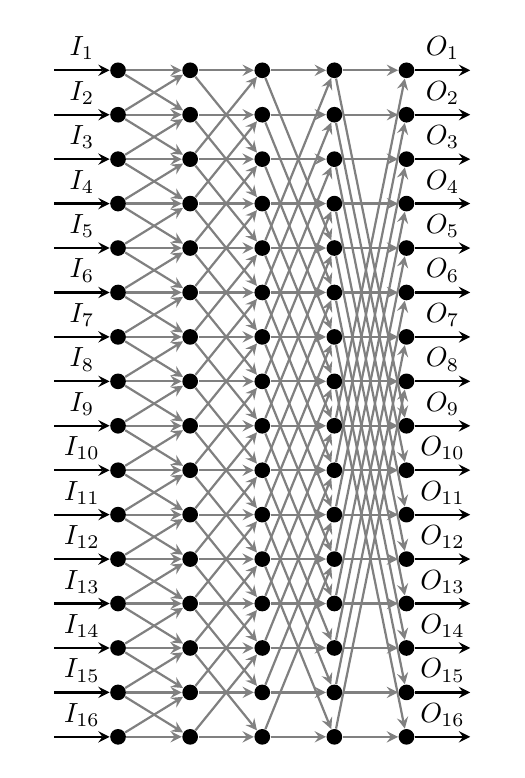
\begin{tikzpicture}[transform shape]
		\node[circle, fill, inner sep=0.2em] (s1) {};
		\node[circle, below=1em of s1, fill, inner sep=0.2em] (s2) {};
		\node[circle, below=1em of s2, fill, inner sep=0.2em] (s3) {};
		\node[circle, below=1em of s3, fill, inner sep=0.2em] (s4) {};
		\node[circle, below=1em of s4, fill, inner sep=0.2em] (s5) {};
		\node[circle, below=1em of s5, fill, inner sep=0.2em] (s6) {};
		\node[circle, below=1em of s6, fill, inner sep=0.2em] (s7) {};
		\node[circle, below=1em of s7, fill, inner sep=0.2em] (s8) {};
		\node[circle, below=1em of s8, fill, inner sep=0.2em] (s9) {};
		\node[circle, below=1em of s9, fill, inner sep=0.2em] (s10) {};
		\node[circle, below=1em of s10, fill, inner sep=0.2em] (s11) {};
		\node[circle, below=1em of s11, fill, inner sep=0.2em] (s12) {};
		\node[circle, below=1em of s12, fill, inner sep=0.2em] (s13) {};
		\node[circle, below=1em of s13, fill, inner sep=0.2em] (s14) {};
		\node[circle,below=1em of s14,  fill, inner sep=0.2em] (s15) {};
		\node[circle, below=1em of s15, fill, inner sep=0.2em] (s16) {};
		
		\foreach \x in {1,...,16}
    		\node[circle, right=2em of s\x, fill, inner sep=0.2em] (h\x) {};
		\foreach \x in {1,...,16}
    		\node[circle, right=2em of h\x, fill, inner sep=0.2em] (hh\x) {};
		\foreach \x in {1,...,16}
    		\node[circle, right=2em of hh\x, fill, inner sep=0.2em] (hhh\x) {};
		\foreach \x in {1,...,16}
    		\node[circle, right=2em of hhh\x, fill, inner sep=0.2em] (hhhh\x) {};
		\foreach \x in {1,...,16}
    		\node[circle, right=2em of hhhh\x] (o\x) {};
		\foreach \x in {1,...,16}
    		\node[circle, left=2em of s\x] (i\x) {};
    		
		\foreach \x in {1,...,16}
    		\draw[-stealth, thick] (i\x) --node[above] {$I_{\x}$} (s\x);
		\foreach \x in {1,...,16}
    		\draw[-stealth, thick] (hhhh\x) --node[above] {$O_{\x}$} (o\x);
		\foreach \x in {1,...,16}
    		\draw[-stealth, thick, gray] (s\x) -- (h\x);
		\foreach \x in {1,...,16}
    		\draw[-stealth, thick, gray] (h\x) -- (hh\x);
		\foreach \x in {1,...,16}
    		\draw[-stealth, thick, gray] (hh\x) -- (hhh\x);
		\foreach \x in {1,...,16}
    		\draw[-stealth, thick, gray] (hhh\x) -- (hhhh\x);
    		
    	\draw[-stealth, thick, gray] (s1) -- (h2);
    	\draw[-stealth, thick, gray] (s2) -- (h1);
    	\draw[-stealth, thick, gray] (s2) -- (h3);
    	\draw[-stealth, thick, gray] (s3) -- (h2);
    	\draw[-stealth, thick, gray] (s3) -- (h4);
    	\draw[-stealth, thick, gray] (s4) -- (h3);
    	\draw[-stealth, thick, gray] (s4) -- (h5);
    	\draw[-stealth, thick, gray] (s5) -- (h4);
    	\draw[-stealth, thick, gray] (s5) -- (h6);
    	\draw[-stealth, thick, gray] (s6) -- (h5);
    	\draw[-stealth, thick, gray] (s6) -- (h7);
    	\draw[-stealth, thick, gray] (s7) -- (h6);
    	\draw[-stealth, thick, gray] (s7) -- (h8);
    	\draw[-stealth, thick, gray] (s8) -- (h7);
    	\draw[-stealth, thick, gray] (s8) -- (h9);
    	\draw[-stealth, thick, gray] (s9) -- (h8);
    	\draw[-stealth, thick, gray] (s9) -- (h10);
    	\draw[-stealth, thick, gray] (s10) -- (h9);
    	\draw[-stealth, thick, gray] (s10) -- (h11);
    	\draw[-stealth, thick, gray] (s11) -- (h10);
    	\draw[-stealth, thick, gray] (s11) -- (h12);
    	\draw[-stealth, thick, gray] (s12) -- (h11);
    	\draw[-stealth, thick, gray] (s12) -- (h13);
    	\draw[-stealth, thick, gray] (s13) -- (h12);
    	\draw[-stealth, thick, gray] (s13) -- (h14);
    	\draw[-stealth, thick, gray] (s14) -- (h13);
    	\draw[-stealth, thick, gray] (s14) -- (h15);
    	\draw[-stealth, thick, gray] (s15) -- (h14);
    	\draw[-stealth, thick, gray] (s15) -- (h16);
    	\draw[-stealth, thick, gray] (s16) -- (h15);
    	
    	
    	\draw[-stealth, thick, gray] (h1) -- (hh3);
    	\draw[-stealth, thick, gray] (h2) -- (hh4);
    	\draw[-stealth, thick, gray] (h3) -- (hh1);
    	\draw[-stealth, thick, gray] (h3) -- (hh5);
    	\draw[-stealth, thick, gray] (h4) -- (hh2);
    	\draw[-stealth, thick, gray] (h4) -- (hh6);
    	\draw[-stealth, thick, gray] (h5) -- (hh3);
    	\draw[-stealth, thick, gray] (h5) -- (hh7);
    	\draw[-stealth, thick, gray] (h6) -- (hh4);
    	\draw[-stealth, thick, gray] (h6) -- (hh8);
    	\draw[-stealth, thick, gray] (h7) -- (hh5);
    	\draw[-stealth, thick, gray] (h7) -- (hh9);
    	\draw[-stealth, thick, gray] (h8) -- (hh6);
    	\draw[-stealth, thick, gray] (h8) -- (hh10);
    	\draw[-stealth, thick, gray] (h9) -- (hh7);
    	\draw[-stealth, thick, gray] (h9) -- (hh11);
    	\draw[-stealth, thick, gray] (h10) -- (hh8);
    	\draw[-stealth, thick, gray] (h10) -- (hh12);
    	\draw[-stealth, thick, gray] (h11) -- (hh9);
    	\draw[-stealth, thick, gray] (h11) -- (hh13);
    	\draw[-stealth, thick, gray] (h12) -- (hh10);
    	\draw[-stealth, thick, gray] (h12) -- (hh14);
    	\draw[-stealth, thick, gray] (h13) -- (hh11);
    	\draw[-stealth, thick, gray] (h13) -- (hh15);
    	\draw[-stealth, thick, gray] (h14) -- (hh12);
    	\draw[-stealth, thick, gray] (h14) -- (hh16);
    	\draw[-stealth, thick, gray] (h15) -- (hh13);
    	\draw[-stealth, thick, gray] (h16) -- (hh14);
    	
    	\draw[-stealth, thick, gray] (hh1) -- (hhh5);
    	\draw[-stealth, thick, gray] (hh2) -- (hhh6);
    	\draw[-stealth, thick, gray] (hh3) -- (hhh7);
    	\draw[-stealth, thick, gray] (hh4) -- (hhh8);
    	\draw[-stealth, thick, gray] (hh5) -- (hhh1);
    	\draw[-stealth, thick, gray] (hh5) -- (hhh9);
    	\draw[-stealth, thick, gray] (hh6) -- (hhh2);
    	\draw[-stealth, thick, gray] (hh6) -- (hhh10);
    	\draw[-stealth, thick, gray] (hh7) -- (hhh3);
    	\draw[-stealth, thick, gray] (hh7) -- (hhh11);
    	\draw[-stealth, thick, gray] (hh8) -- (hhh4);
    	\draw[-stealth, thick, gray] (hh8) -- (hhh12);
    	\draw[-stealth, thick, gray] (hh9) -- (hhh5);
    	\draw[-stealth, thick, gray] (hh9) -- (hhh13);
    	\draw[-stealth, thick, gray] (hh10) -- (hhh6);
    	\draw[-stealth, thick, gray] (hh10) -- (hhh14);
    	\draw[-stealth, thick, gray] (hh11) -- (hhh7);
    	\draw[-stealth, thick, gray] (hh11) -- (hhh15);
    	\draw[-stealth, thick, gray] (hh12) -- (hhh8);
    	\draw[-stealth, thick, gray] (hh12) -- (hhh16);
    	\draw[-stealth, thick, gray] (hh13) -- (hhh9);
    	\draw[-stealth, thick, gray] (hh14) -- (hhh10);
    	\draw[-stealth, thick, gray] (hh15) -- (hhh11);
    	\draw[-stealth, thick, gray] (hh16) -- (hhh12);
    	
    	\draw[-stealth, thick, gray] (hhh1) -- (hhhh9);
    	\draw[-stealth, thick, gray] (hhh2) -- (hhhh10);
    	\draw[-stealth, thick, gray] (hhh3) -- (hhhh11);
    	\draw[-stealth, thick, gray] (hhh4) -- (hhhh12);
    	\draw[-stealth, thick, gray] (hhh5) -- (hhhh13);
    	\draw[-stealth, thick, gray] (hhh6) -- (hhhh14);
    	\draw[-stealth, thick, gray] (hhh7) -- (hhhh15);
    	\draw[-stealth, thick, gray] (hhh8) -- (hhhh16);
    	\draw[-stealth, thick, gray] (hhh9) -- (hhhh1);
    	\draw[-stealth, thick, gray] (hhh10) -- (hhhh2);
    	\draw[-stealth, thick, gray] (hhh11) -- (hhhh3);
    	\draw[-stealth, thick, gray] (hhh12) -- (hhhh4);
    	\draw[-stealth, thick, gray] (hhh13) -- (hhhh5);
    	\draw[-stealth, thick, gray] (hhh14) -- (hhhh6);
    	\draw[-stealth, thick, gray] (hhh15) -- (hhhh7);
    	\draw[-stealth, thick, gray] (hhh16) -- (hhhh8);
  	\end{tikzpicture}
  	\end{turn}
	\end{center}
\end{frame}

\begin{frame}
	\frametitle{Temporal dependencies captured by $O_{16}$}	
	\begin{center}
	\begin{turn}{90}
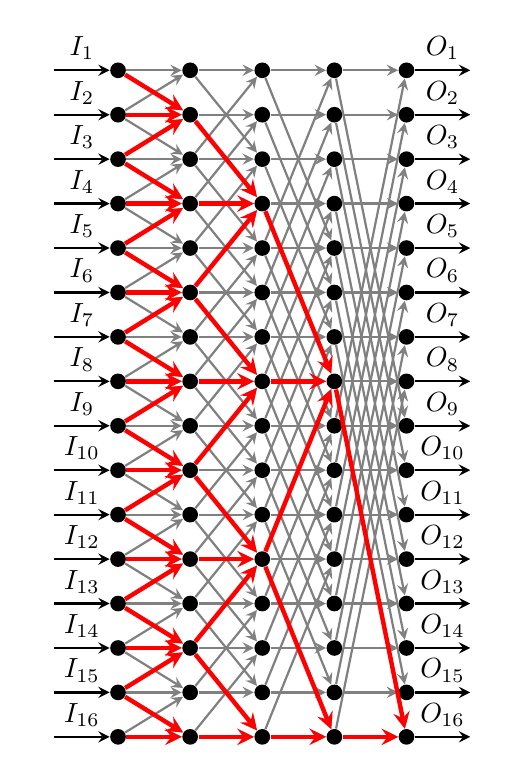
\begin{tikzpicture}[transform shape]
		\node[circle, fill, inner sep=0.2em] (s1) {};
		\node[circle, below=1em of s1, fill, inner sep=0.2em] (s2) {};
		\node[circle, below=1em of s2, fill, inner sep=0.2em] (s3) {};
		\node[circle, below=1em of s3, fill, inner sep=0.2em] (s4) {};
		\node[circle, below=1em of s4, fill, inner sep=0.2em] (s5) {};
		\node[circle, below=1em of s5, fill, inner sep=0.2em] (s6) {};
		\node[circle, below=1em of s6, fill, inner sep=0.2em] (s7) {};
		\node[circle, below=1em of s7, fill, inner sep=0.2em] (s8) {};
		\node[circle, below=1em of s8, fill, inner sep=0.2em] (s9) {};
		\node[circle, below=1em of s9, fill, inner sep=0.2em] (s10) {};
		\node[circle, below=1em of s10, fill, inner sep=0.2em] (s11) {};
		\node[circle, below=1em of s11, fill, inner sep=0.2em] (s12) {};
		\node[circle, below=1em of s12, fill, inner sep=0.2em] (s13) {};
		\node[circle, below=1em of s13, fill, inner sep=0.2em] (s14) {};
		\node[circle,below=1em of s14,  fill, inner sep=0.2em] (s15) {};
		\node[circle, below=1em of s15, fill, inner sep=0.2em] (s16) {};
		
		\foreach \x in {1,...,16}
    		\node[circle, right=2em of s\x, fill, inner sep=0.2em] (h\x) {};
		\foreach \x in {1,...,16}
    		\node[circle, right=2em of h\x, fill, inner sep=0.2em] (hh\x) {};
		\foreach \x in {1,...,16}
    		\node[circle, right=2em of hh\x, fill, inner sep=0.2em] (hhh\x) {};
		\foreach \x in {1,...,16}
    		\node[circle, right=2em of hhh\x, fill, inner sep=0.2em] (hhhh\x) {};
		\foreach \x in {1,...,16}
    		\node[circle, right=2em of hhhh\x] (o\x) {};
		\foreach \x in {1,...,16}
    		\node[circle, left=2em of s\x] (i\x) {};
    		
		\foreach \x in {1,...,16}
    		\draw[-stealth, thick] (i\x) --node[above] {$I_{\x}$} (s\x);
		\foreach \x in {1,...,16}
    		\draw[-stealth, thick] (hhhh\x) --node[above] {$O_{\x}$} (o\x);
		\foreach \x in {1,...,16}
    		\draw[-stealth, thick, gray] (s\x) -- (h\x);
		\foreach \x in {1,...,16}
    		\draw[-stealth, thick, gray] (h\x) -- (hh\x);
		\foreach \x in {1,...,16}
    		\draw[-stealth, thick, gray] (hh\x) -- (hhh\x);
		\foreach \x in {1,...,16}
    		\draw[-stealth, thick, gray] (hhh\x) -- (hhhh\x);
    		
    	\draw[-stealth, thick, gray] (s1) -- (h2);
    	\draw[-stealth, thick, gray] (s2) -- (h1);
    	\draw[-stealth, thick, gray] (s2) -- (h3);
    	\draw[-stealth, thick, gray] (s3) -- (h2);
    	\draw[-stealth, thick, gray] (s3) -- (h4);
    	\draw[-stealth, thick, gray] (s4) -- (h3);
    	\draw[-stealth, thick, gray] (s4) -- (h5);
    	\draw[-stealth, thick, gray] (s5) -- (h4);
    	\draw[-stealth, thick, gray] (s5) -- (h6);
    	\draw[-stealth, thick, gray] (s6) -- (h5);
    	\draw[-stealth, thick, gray] (s6) -- (h7);
    	\draw[-stealth, thick, gray] (s7) -- (h6);
    	\draw[-stealth, thick, gray] (s7) -- (h8);
    	\draw[-stealth, thick, gray] (s8) -- (h7);
    	\draw[-stealth, thick, gray] (s8) -- (h9);
    	\draw[-stealth, thick, gray] (s9) -- (h8);
    	\draw[-stealth, thick, gray] (s9) -- (h10);
    	\draw[-stealth, thick, gray] (s10) -- (h9);
    	\draw[-stealth, thick, gray] (s10) -- (h11);
    	\draw[-stealth, thick, gray] (s11) -- (h10);
    	\draw[-stealth, thick, gray] (s11) -- (h12);
    	\draw[-stealth, thick, gray] (s12) -- (h11);
    	\draw[-stealth, thick, gray] (s12) -- (h13);
    	\draw[-stealth, thick, gray] (s13) -- (h12);
    	\draw[-stealth, thick, gray] (s13) -- (h14);
    	\draw[-stealth, thick, gray] (s14) -- (h13);
    	\draw[-stealth, thick, gray] (s14) -- (h15);
    	\draw[-stealth, thick, gray] (s15) -- (h14);
    	\draw[-stealth, thick, gray] (s15) -- (h16);
    	\draw[-stealth, thick, gray] (s16) -- (h15);
    	
    	
    	\draw[-stealth, thick, gray] (h1) -- (hh3);
    	\draw[-stealth, thick, gray] (h2) -- (hh4);
    	\draw[-stealth, thick, gray] (h3) -- (hh1);
    	\draw[-stealth, thick, gray] (h3) -- (hh5);
    	\draw[-stealth, thick, gray] (h4) -- (hh2);
    	\draw[-stealth, thick, gray] (h4) -- (hh6);
    	\draw[-stealth, thick, gray] (h5) -- (hh3);
    	\draw[-stealth, thick, gray] (h5) -- (hh7);
    	\draw[-stealth, thick, gray] (h6) -- (hh4);
    	\draw[-stealth, thick, gray] (h6) -- (hh8);
    	\draw[-stealth, thick, gray] (h7) -- (hh5);
    	\draw[-stealth, thick, gray] (h7) -- (hh9);
    	\draw[-stealth, thick, gray] (h8) -- (hh6);
    	\draw[-stealth, thick, gray] (h8) -- (hh10);
    	\draw[-stealth, thick, gray] (h9) -- (hh7);
    	\draw[-stealth, thick, gray] (h9) -- (hh11);
    	\draw[-stealth, thick, gray] (h10) -- (hh8);
    	\draw[-stealth, thick, gray] (h10) -- (hh12);
    	\draw[-stealth, thick, gray] (h11) -- (hh9);
    	\draw[-stealth, thick, gray] (h11) -- (hh13);
    	\draw[-stealth, thick, gray] (h12) -- (hh10);
    	\draw[-stealth, thick, gray] (h12) -- (hh14);
    	\draw[-stealth, thick, gray] (h13) -- (hh11);
    	\draw[-stealth, thick, gray] (h13) -- (hh15);
    	\draw[-stealth, thick, gray] (h14) -- (hh12);
    	\draw[-stealth, thick, gray] (h14) -- (hh16);
    	\draw[-stealth, thick, gray] (h15) -- (hh13);
    	\draw[-stealth, thick, gray] (h16) -- (hh14);
    	
    	\draw[-stealth, thick, gray] (hh1) -- (hhh5);
    	\draw[-stealth, thick, gray] (hh2) -- (hhh6);
    	\draw[-stealth, thick, gray] (hh3) -- (hhh7);
    	\draw[-stealth, thick, gray] (hh4) -- (hhh8);
    	\draw[-stealth, thick, gray] (hh5) -- (hhh1);
    	\draw[-stealth, thick, gray] (hh5) -- (hhh9);
    	\draw[-stealth, thick, gray] (hh6) -- (hhh2);
    	\draw[-stealth, thick, gray] (hh6) -- (hhh10);
    	\draw[-stealth, thick, gray] (hh7) -- (hhh3);
    	\draw[-stealth, thick, gray] (hh7) -- (hhh11);
    	\draw[-stealth, thick, gray] (hh8) -- (hhh4);
    	\draw[-stealth, thick, gray] (hh8) -- (hhh12);
    	\draw[-stealth, thick, gray] (hh9) -- (hhh5);
    	\draw[-stealth, thick, gray] (hh9) -- (hhh13);
    	\draw[-stealth, thick, gray] (hh10) -- (hhh6);
    	\draw[-stealth, thick, gray] (hh10) -- (hhh14);
    	\draw[-stealth, thick, gray] (hh11) -- (hhh7);
    	\draw[-stealth, thick, gray] (hh11) -- (hhh15);
    	\draw[-stealth, thick, gray] (hh12) -- (hhh8);
    	\draw[-stealth, thick, gray] (hh12) -- (hhh16);
    	\draw[-stealth, thick, gray] (hh13) -- (hhh9);
    	\draw[-stealth, thick, gray] (hh14) -- (hhh10);
    	\draw[-stealth, thick, gray] (hh15) -- (hhh11);
    	\draw[-stealth, thick, gray] (hh16) -- (hhh12);
    	
    	\draw[-stealth, thick, gray] (hhh1) -- (hhhh9);
    	\draw[-stealth, thick, gray] (hhh2) -- (hhhh10);
    	\draw[-stealth, thick, gray] (hhh3) -- (hhhh11);
    	\draw[-stealth, thick, gray] (hhh4) -- (hhhh12);
    	\draw[-stealth, thick, gray] (hhh5) -- (hhhh13);
    	\draw[-stealth, thick, gray] (hhh6) -- (hhhh14);
    	\draw[-stealth, thick, gray] (hhh7) -- (hhhh15);
    	\draw[-stealth, thick, gray] (hhh8) -- (hhhh16);
    	\draw[-stealth, thick, gray] (hhh9) -- (hhhh1);
    	\draw[-stealth, thick, gray] (hhh10) -- (hhhh2);
    	\draw[-stealth, thick, gray] (hhh11) -- (hhhh3);
    	\draw[-stealth, thick, gray] (hhh12) -- (hhhh4);
    	\draw[-stealth, thick, gray] (hhh13) -- (hhhh5);
    	\draw[-stealth, thick, gray] (hhh14) -- (hhhh6);
    	\draw[-stealth, thick, gray] (hhh15) -- (hhhh7);
    	\draw[-stealth, thick, gray] (hhh16) -- (hhhh8);
    	
    	\draw[-stealth, ultra thick, red] (hhh16) -- (hhhh16);
    	\draw[-stealth, ultra thick, red] (hhh8) -- (hhhh16);
    	
    	\draw[-stealth, ultra thick, red] (hh16) -- (hhh16);
    	\draw[-stealth, ultra thick, red] (hh12) -- (hhh16);
    	\draw[-stealth, ultra thick, red] (hh4) -- (hhh8);
    	\draw[-stealth, ultra thick, red] (hh8) -- (hhh8);
    	\draw[-stealth, ultra thick, red] (hh12) -- (hhh8);
    	
    	\draw[-stealth, ultra thick, red] (h16) -- (hh16);
    	\draw[-stealth, ultra thick, red] (h14) -- (hh16);
    	\draw[-stealth, ultra thick, red] (h14) -- (hh12);
    	\draw[-stealth, ultra thick, red] (h12) -- (hh12);
    	\draw[-stealth, ultra thick, red] (h10) -- (hh12);
    	\draw[-stealth, ultra thick, red] (h10) -- (hh8);
    	\draw[-stealth, ultra thick, red] (h8) -- (hh8);
    	\draw[-stealth, ultra thick, red] (h6) -- (hh8);
    	\draw[-stealth, ultra thick, red] (h6) -- (hh4);
    	\draw[-stealth, ultra thick, red] (h4) -- (hh4);
    	\draw[-stealth, ultra thick, red] (h2) -- (hh4);
    	
    	\draw[-stealth, ultra thick, red] (s16) -- (h16);
    	\draw[-stealth, ultra thick, red] (s15) -- (h16);
    	\draw[-stealth, ultra thick, red] (s15) -- (h14);
    	\draw[-stealth, ultra thick, red] (s14) -- (h14);
    	\draw[-stealth, ultra thick, red] (s13) -- (h14);
    	\draw[-stealth, ultra thick, red] (s13) -- (h12);
    	\draw[-stealth, ultra thick, red] (s12) -- (h12);
    	\draw[-stealth, ultra thick, red] (s11) -- (h12);
    	\draw[-stealth, ultra thick, red] (s11) -- (h10);
    	\draw[-stealth, ultra thick, red] (s10) -- (h10);
    	\draw[-stealth, ultra thick, red] (s9) -- (h10);
    	\draw[-stealth, ultra thick, red] (s9) -- (h8);
    	\draw[-stealth, ultra thick, red] (s8) -- (h8);
    	\draw[-stealth, ultra thick, red] (s7) -- (h8);
    	\draw[-stealth, ultra thick, red] (s7) -- (h6);
    	\draw[-stealth, ultra thick, red] (s6) -- (h6);
    	\draw[-stealth, ultra thick, red] (s5) -- (h6);
    	\draw[-stealth, ultra thick, red] (s5) -- (h4);
    	\draw[-stealth, ultra thick, red] (s4) -- (h4);
    	\draw[-stealth, ultra thick, red] (s3) -- (h4);
    	\draw[-stealth, ultra thick, red] (s3) -- (h2);
    	\draw[-stealth, ultra thick, red] (s2) -- (h2);
    	\draw[-stealth, ultra thick, red] (s1) -- (h2);
  	\end{tikzpicture}
  	\end{turn}
	\end{center}
\end{frame}


\begin{frame}
	\frametitle{Thank you!}
    \centering
    {\Huge Questions?}\\ \hfill \\
    {\tt \LARGE petar.velickovic@cl.cam.ac.uk}\\ \hfill \\
    {\tt \large https://github.com/PetarV-/a-trip-down-lstm-lane}
\end{frame}


\end{document}


